%% This is file `DEMO-TUDaThesis.tex' version 3.32 (2023/06/19),
%% it is part of
%% TUDa-CI -- Corporate Design for TU Darmstadt
%% ----------------------------------------------------------------------------
%%
%%  Copyright (C) 2018--2023 by Marei Peischl <marei@peitex.de>
%%
%% ============================================================================
%% This work may be distributed and/or modified under the
%% conditions of the LaTeX Project Public License, either version 1.3c
%% of this license or (at your option) any later version.
%% The latest version of this license is in
%% http://www.latex-project.org/lppl.txt
%% and version 1.3c or later is part of all distributions of LaTeX
%% version 2008/05/04 or later.
%%
%% This work has the LPPL maintenance status `maintained'.
%%
%% The Current Maintainers of this work are
%%   Marei Peischl <tuda-ci@peitex.de>
%%   Markus Lazanowski <latex@ce.tu-darmstadt.de>
%%
%% The development respository can be found at
%% https://github.com/tudace/tuda_latex_templates
%% Please use the issue tracker for feedback!
%%
%% If you need a compiled version of this document, have a look at
%% http://mirror.ctan.org/macros/latex/contrib/tuda-ci/doc
%% or at the documentation directory of this package (if installed)
%% <path to your LaTeX distribution>/doc/latex/tuda-ci
%% ============================================================================
%%
% !TeX program = lualatex
%%

\documentclass[
	ngerman,
	ruledheaders=section,%Ebene bis zu der die Überschriften mit Linien abgetrennt werden, vgl. DEMO-TUDaPub
	class=report,% Basisdokumentenklasse. Wählt die Korrespondierende KOMA-Script Klasse
	thesis={type=master},% Dokumententyp Thesis, für Dissertationen siehe die Demo-Datei DEMO-TUDaPhd
	accentcolor=9c,% Auswahl der Akzentfarbe
	custommargins=true,% Ränder werden mithilfe von typearea automatisch berechnet
	marginpar=false,% Kopfzeile und Fußzeile erstrecken sich nicht über die Randnotizspalte
	%BCOR=5mm,%Bindekorrektur, falls notwendig
	parskip=half-,%Absatzkennzeichnung durch Abstand vgl. KOMA-Script
	fontsize=11pt,%Basisschriftgröße laut Corporate Design ist mit 9pt häufig zu klein
	%	logofile=example-image, %Falls die Logo Dateien nicht vorliegen
]{tudapub}


% Der folgende Block ist nur bei pdfTeX auf Versionen vor April 2018 notwendig
\usepackage{iftex}
\ifPDFTeX
	\usepackage[utf8]{inputenc}%kompatibilität mit TeX Versionen vor April 2018
\fi

%%%%%%%%%%%%%%%%%%%
%Sprachanpassung & Verbesserte Trennregeln
%%%%%%%%%%%%%%%%%%%
\usepackage[ngerman, main=english]{babel}
\usepackage[autostyle]{csquotes}% Anführungszeichen vereinfacht

% Falls mit pdflatex kompiliert wird, wird microtype automatisch geladen, in diesem Fall muss diese Zeile entfernt werden, und falls weiter Optionen hinzugefügt werden sollen, muss dies über
% \PassOptionsToPackage{Optionen}{microtype}
% vor \documentclass hinzugefügt werden.
\usepackage{microtype}

%%%%%%%%%%%%%%%%%%%
%Literaturverzeichnis
%%%%%%%%%%%%%%%%%%%
\usepackage{biblatex}   % Literaturverzeichnis
%\bibliography{DEMO-TUDaBibliography.bib}
\addbibresource{biblio.bib}
\setcounter{tocdepth}{4}
\setcounter{secnumdepth}{4}


%%%%%%%%%%%%%%%%%%%
%Paketvorschläge Tabellen
%%%%%%%%%%%%%%%%%%%
%\usepackage{array}     % Basispaket für Tabellenkonfiguration, wird von den folgenden automatisch geladen
\usepackage{tabularx}   % Tabellen, die sich automatisch der Breite anpassen
%\usepackage{longtable} % Mehrseitige Tabellen
%\usepackage{xltabular} % Mehrseitige Tabellen mit anpassbarer Breite
\usepackage{booktabs}   % Verbesserte Möglichkeiten für Tabellenlayout über horizontale Linien
\usepackage{float}
\usepackage{amsmath}

%%%%%%%%%%%%%%%%%%%
%Paketvorschläge Mathematik
%%%%%%%%%%%%%%%%%%%
%\usepackage{mathtools} % erweiterte Fassung von amsmath
%\usepackage{amssymb}   % erweiterter Zeichensatz
%\usepackage{siunitx}   % Einheiten

%Formatierungen für Beispiele in diesem Dokument. Im Allgemeinen nicht notwendig!
\let\file\texttt
\let\code\texttt
\let\tbs\textbackslash
\let\pck\textsf
\let\cls\textsf

\usepackage{pifont}% Zapf-Dingbats Symbole
\newcommand*{\FeatureTrue}{\ding{52}}
\newcommand*{\FeatureFalse}{\ding{56}}

\begin{document}

\Metadata{
	title=Thesis,
	author=Denis Andrić
}

\title{Implementation of Neural Models for Accurate Prediction of Robot Trajectories in Hamiltonian Spaces: A Graph Neural Network Approach}
\subtitle{Implementierung von neuronalen Modellen zur präzisen Vorhersage von Trajektorien in Hamiltonschen Räumen: 
	Ein Ansatz mit Graph-Neuronalen Netzwerken}
\author[D. Andrić]{Denis Andrić}
\studentID{2486004}%optionales Argument ist die Signatur,
\birthplace{Darmstadt}%Geburtsort, bei Dissertationen zwingend notwendig
\reviewer{Georgia Chalvatzaki \and An Thai Le}%Gutachter

%Diese Felder werden untereinander auf der Titelseite platziert.
%\department ist eine notwendige Angabe, siehe auch dem Abschnitt `Abweichung von den Vorgaben für die Titelseite'
%\department{ce} % Das Kürzel wird automatisch ersetzt und als Studienfach gewählt, siehe Liste der Kürzel im Dokument.
%\institute{FB 20}
\addTitleBoxLogo*{
\includegraphics[width=0.5\linewidth]{logos/CELogo.png}}
\addTitleBoxLogo*{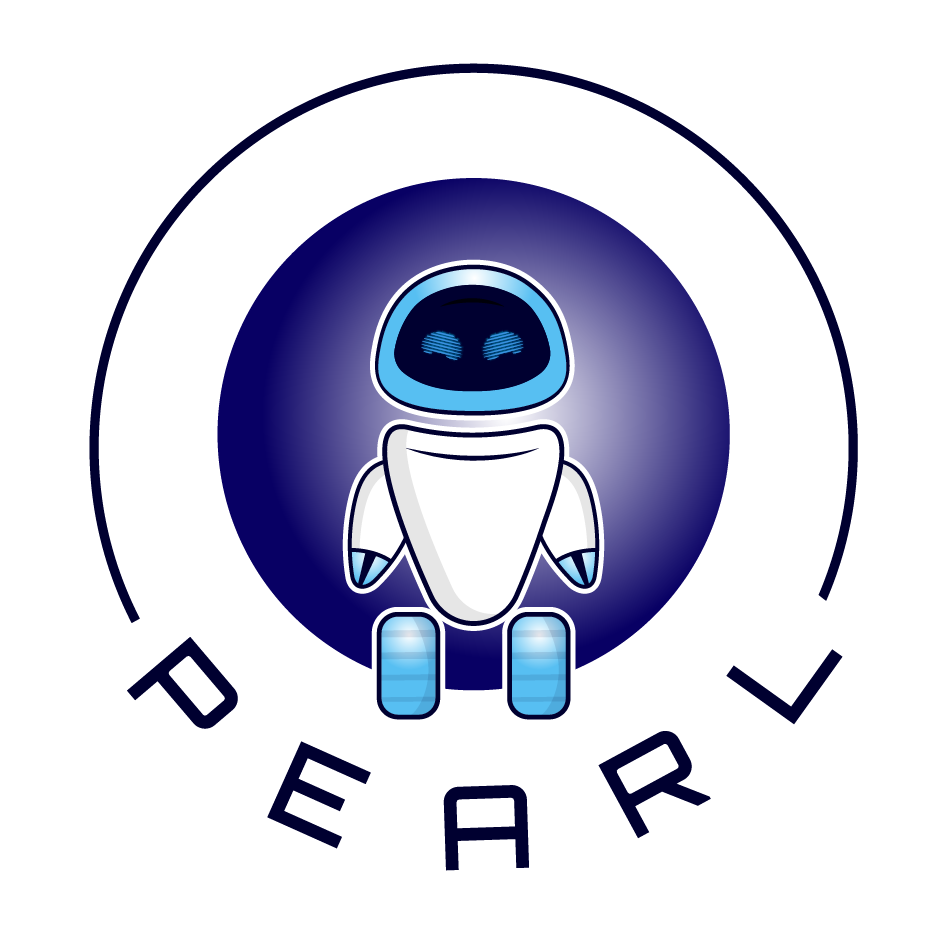
\includegraphics[width=0.5\linewidth]{logos/pearllogo.png}}
\addTitleBoxLogo*{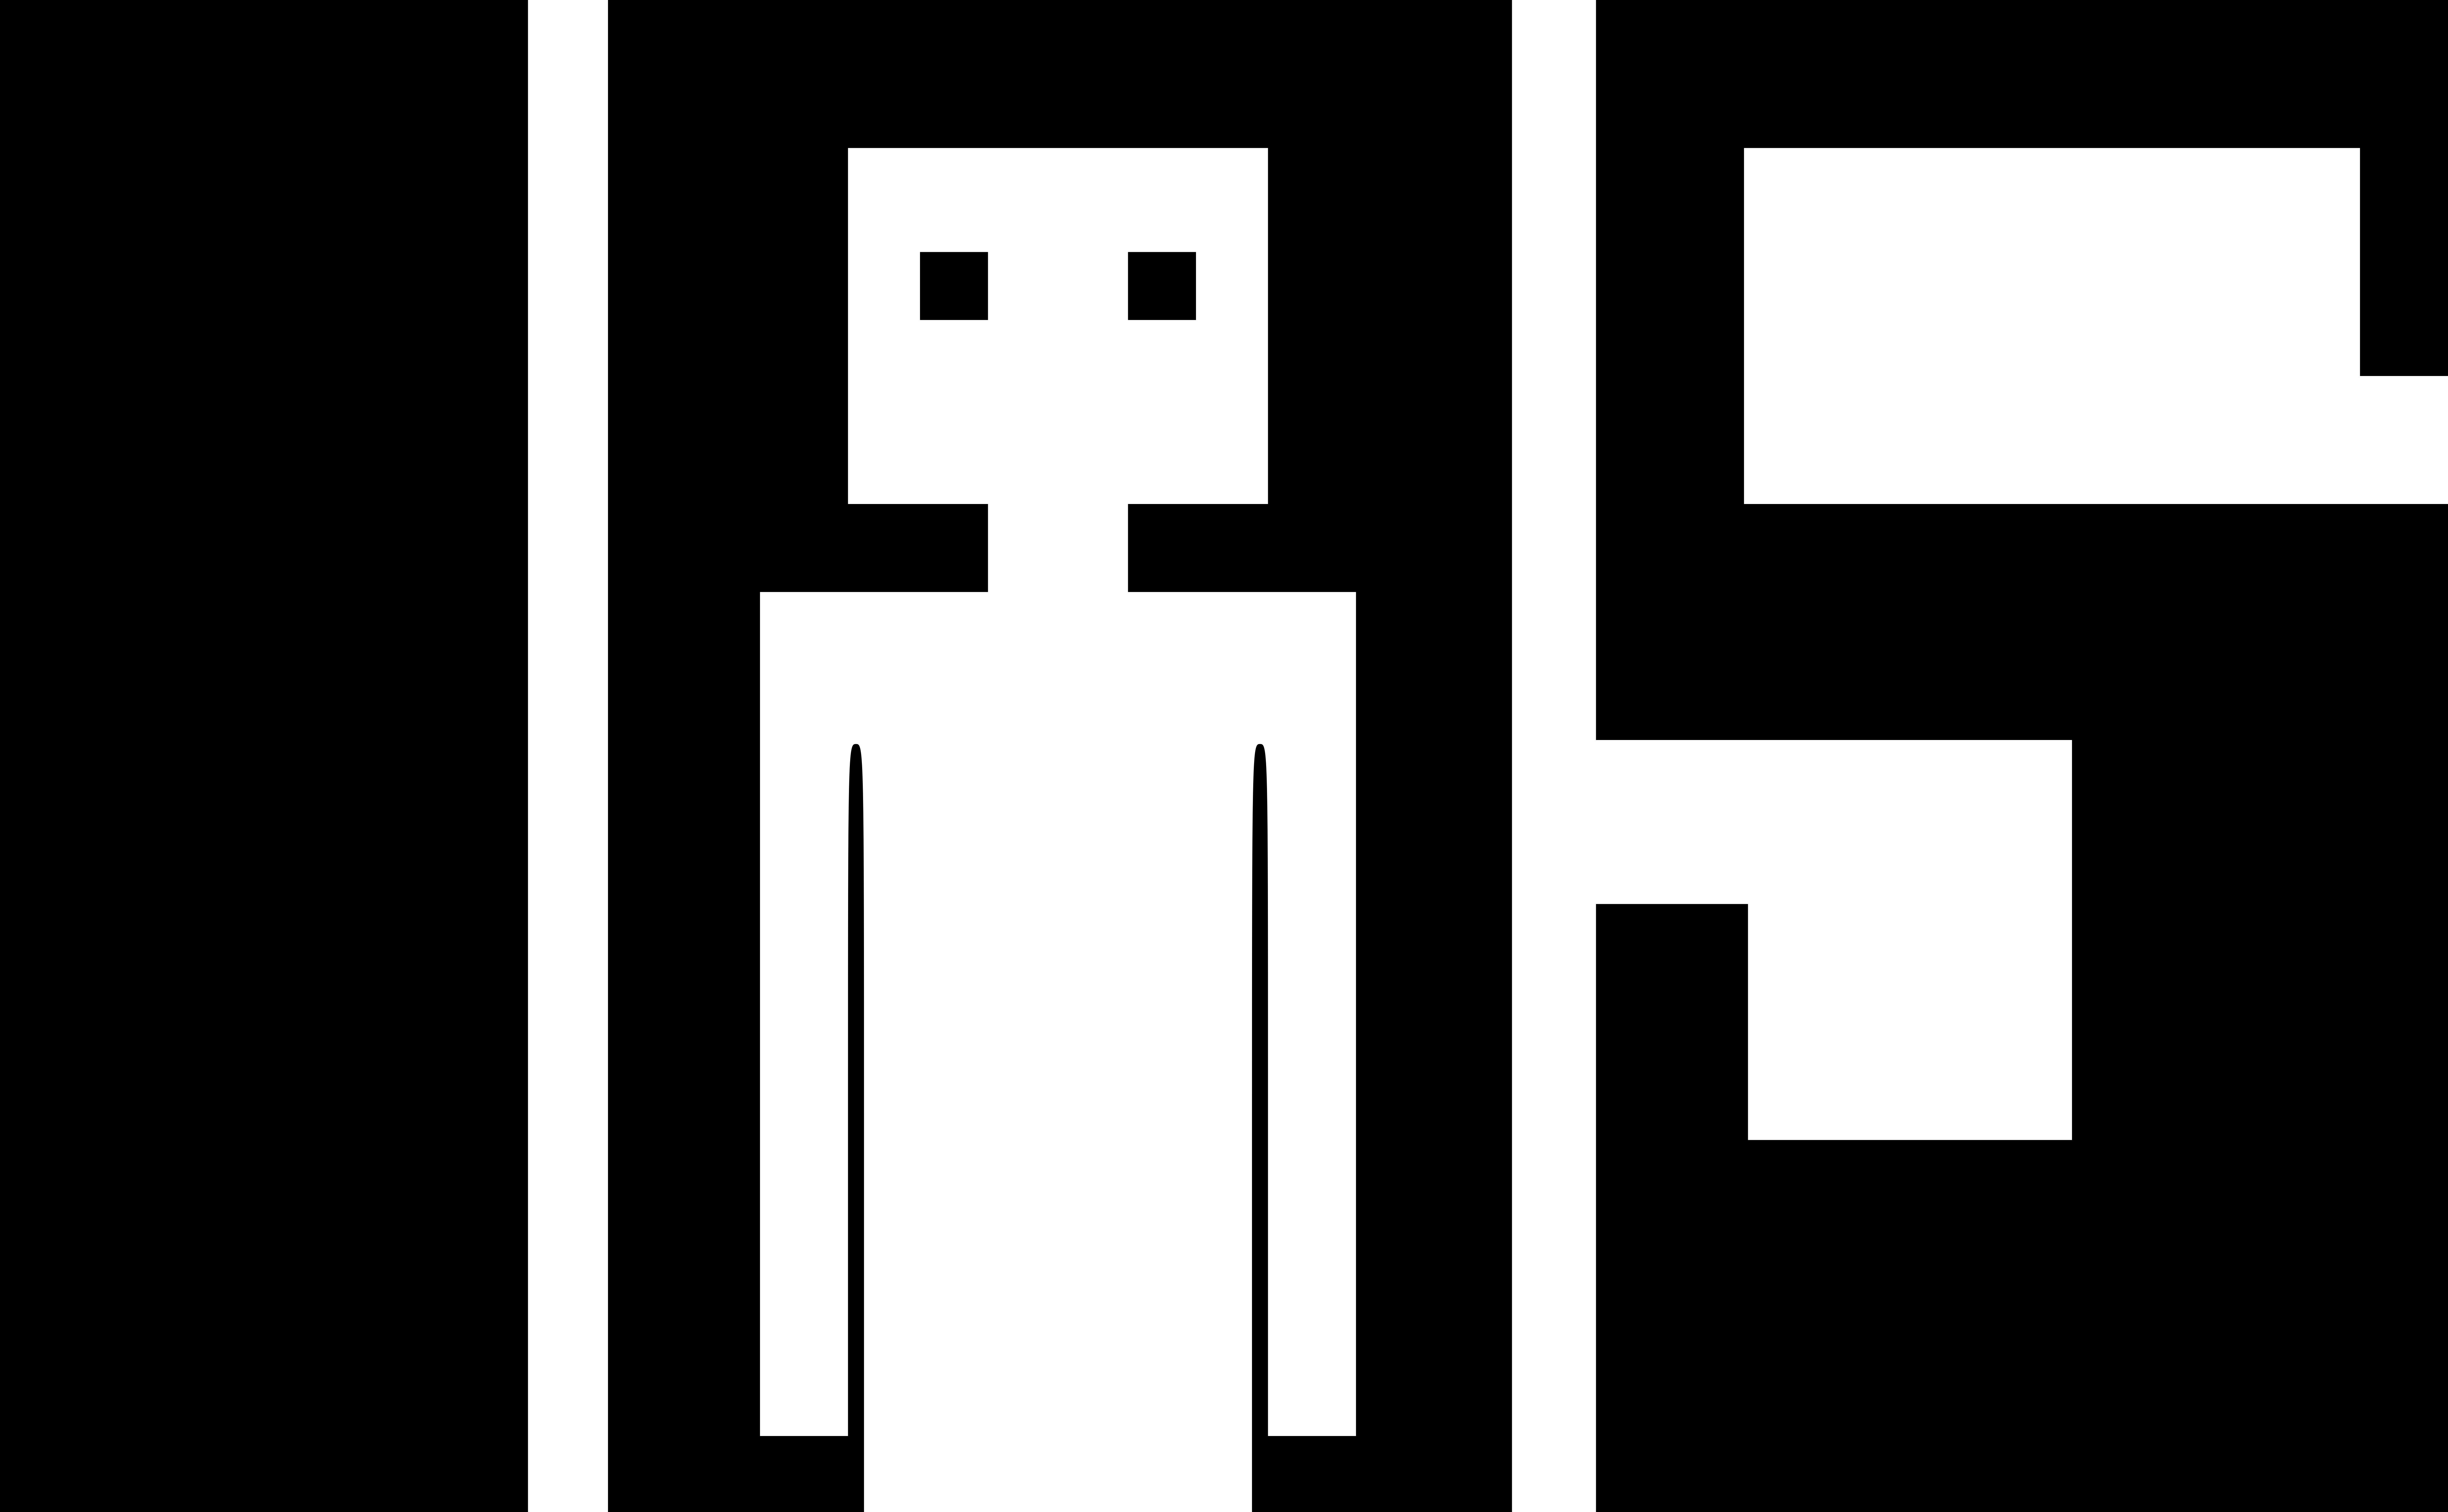
\includegraphics[width=0.5\linewidth]{logos/iasLogo.png}}
\submissiondate{\today}
\examdate{\today}

% Hinweis zur Lizenz:
% TUDa-CI verwendet momentan die Lizenz CC BY-NC-ND 2.0 DE als Voreinstellung.
% Die TU Darmstadt hat jedoch die Empfehlung von dieser auf die liberalere
% CC BY 4.0 geändert. Diese erlaubt eine Verwendung bearbeiteter Versionen und
% die kommerzielle Nutzung.
% TUDa-CI wird im nächsten größeren Release ebenfalls diese Anpassung vornehmen.
% Aus diesem Grund wird empfohlen die Lizenz manuell auszuwählen.
%\tuprints{urn=XXXXX,printid=XXXX,year=2022,license=cc-by-4.0}
% To see further information on the license option in English, remove the license= key and pay attention to the warning & help message.

% \dedication{Für alle, die \TeX{} nutzen.}

\maketitle

\affidavit
% Es gibt mit Version 3.20 die Möglichkeit ein Bild als Signatur einzubinden.
% TUDa-CI kann nicht garantieren, dass dies zulässig ist oder eine eigenhändige Unterschrift ersetzt.
% Dies ist durch Studierende vor der Verwendung abzuklären.
% Die Verwendung funktioniert so:
%\affidavit[signature-image={\includegraphics[width=\width,height=1cm]{example-image}}, <hier können andere Optionen zusätzlich stehen>]

\tableofcontents
\listoffigures
\listoftables+

\chapter*{Abstract}
The introduction of the adjoint method for NeuralODEs\cite{neuralODE} has created new ways for physics-based trajectory predictions. In the subsequent chapters of this thesis, we look at deep learning models and methods targeted at predicting physical systems' behavior. We use the guiding light of Hamiltonian equations to dive into systems such as the harmonic oscillator and the three-body problem. We are intrigued with exploring graph neural networks' ability to be used in physics informed models: in the N-body problem and in the N-pendulum. This work tests the ability of graph neural networks to generalize the behavior from single realizations of elements at the node level of the graph. In this way, we hope to exemplify how such models can capture highly dynamic physical processes. 


\chapter{Introduction}
The intersection of physics and deep learning has never been more pronounced than it is today. With advancements in hardware and computational capabilities, we are now positioned to predict physical phenomena with unprecedented precision using deep learning techniques, particularly through physics-informed neural networks.\\
Physics-Informed Neural Networks (PINN) are neural networks  that encode model equations, like Partial Differential Equations (PDE), as a component of the neural network itself\cite{}. For example let us take Laplace equation which is defined as
\begin{eqnarray}
	\Delta u(\mathbf{x}) &= 0, &\texttt{   }\mathbf{x}\in \Omega,\mathbf{x}\in R^2\\
	u &= S &\texttt{   }\mathbf{x}\in \partial\Omega \text{     Dirichlet boundary condition},\\
	\frac{\partial u}{\partial \mathbf{n}} &= f(\mathbf{x}) &\texttt{   }\mathbf{x}\in \partial\Omega \text{     Neumann boundary condition}.
\end{eqnarray}
The Operator $\Delta$ is called as Laplace Operator and it defines $\Delta = \sum_i \frac{\partial^2}{\partial^2 x_i}.$\\
To build a PINN model we will use an Neural Network which will learn the solution $u$ and from that output we will calculate all needed derivatives, residuals and other parts for the optimization.

\begin{figure}[h!]
	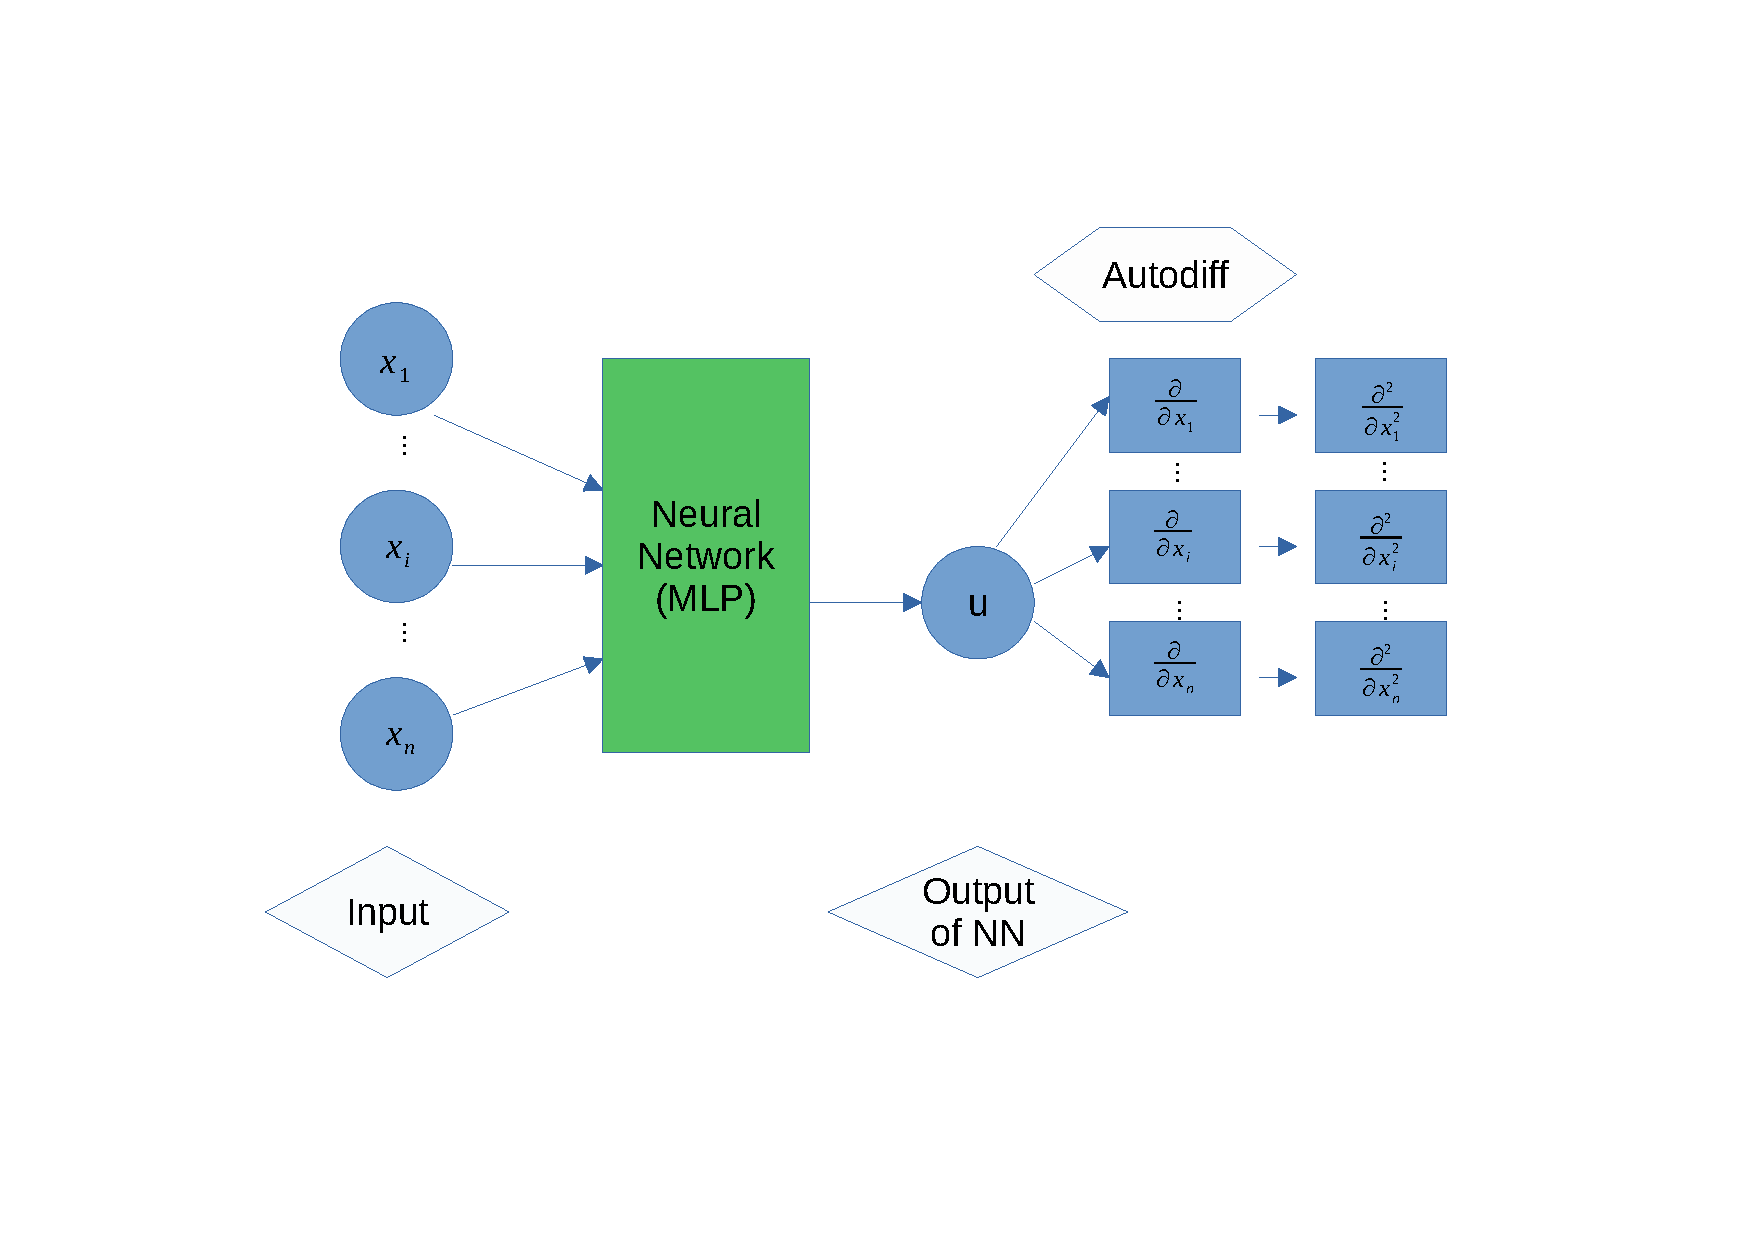
\includegraphics[width=15cm]{chapters/chapter1/pinn}
	\label{pinn}
	\caption{PINN model for Laplace Equation}
\end{figure}
In figure \ref{pinn} we can observe the architecture of such physics informed model. 
The Loss functions that we need to use to properly train our network are
\begin{eqnarray}
	\text{Loss}_s(\Theta) &=& \frac{1}{N}\sum^N_i\left(u_{\Theta}(\mathbf{x}_i)- u_i\right)^2,\\
	\text{Loss}_r(\Theta) &=& \frac{1}{R}\sum^R_i\left(\frac{\partial u_{\Theta}(\mathbf{x}_i)}{\partial x_i} - f(\mathbf{x}_i)\right)^2,\\
	\text{Loss}_l(\Theta) &=& \Delta u_{\Theta},\\
	\text{Loss}(\Theta) &=& \omega_s \text{Loss}_s +\omega_r \text{Loss}_r +\omega_l \text{Loss}_l .
\end{eqnarray}
The $\omega_s$,$\omega_r$,$\omega_l$, in this case are coefficients $0\leq \omega \leq 1$ and they are there to improve optimization capabilities which is defined as
\begin{equation}
	\Theta^* = \arg\min\text{Loss}(\Theta).
\end{equation}
The $\Theta$ are learnable parameters which can be updated with $\Theta^*$ trough optimization algorithm.\\
Such model wouldn't be possible without Automatic Differentiation\cite{} which are offered from machine learning library $\texttt{pytorch}$\cite{}. In this example we need big bunch of data and the optimization of the model could be very slow in addition if we don't have a computation capable hardware for it. Obtaining the data could be done only with exactly measurement or using some numerical solvers like FEM or Isogeometric Analysis. Don't forget, that there are Poission Equation, Wave Equation which are dependent on time $t$.\\
Those PDEs have mostly application in electrotechnical(Electro-magnetical fields) and  civil Engineering(static in construction).
In this thesis we won't work on the PDEs but similar to this topic we will try to train a model to predict the Dynamics of some physical phenomena and non-/holonomic systems of the robots.\\
The Dynamics for Robots are trivially defined as simple Second Level Ordinary Differential Equation\cite{} .
\begin{equation}
	\mathbf{M}\ddot{\mathbf{x}}(t) + \mathbf{D}(\dot{\mathbf{x}}(t)) + \mathbf{C}(\mathbf{x}(t))=0,
\end{equation} but there are other forms, as Langrange Equations of Motion if our system is holonomic\cite{}. It is based on Lagrange Function which is based on Kinetik $T$ and Potential $U$ Energy
\begin{eqnarray}
	\mathcal{L} &=& T - V,\\
	\frac{d}{dt}\frac{\partial \mathcal{L}}{\partial \dot{q}_i} - \frac{\partial \mathcal{L}}{\partial q_i}&=&0.
\end{eqnarray}   
The Lagrange Equations are used in Delan\cite{} Physics informed network and in simillar manner, but for us are most interesting to use Hamiltonian Equations of Motion.
They work for holonomic and non-holonomic systems and they are capable to build First Level Ordinary Equation
\begin{equation}
	\dot{x} = f(x,t)
\end{equation} \\
or in Hamiltonian Form where $\mathcal{H} = T + V$
\begin{equation}
	\dot{\mathbf{z}} = \mathbf{J}\frac{\partial\mathcal{H}}{\partial \mathbf{z}}
\end{equation} where $\mathbf{z}=[\mathbf{q},\mathbf{p}]^T$ and $\mathbf{J} = \begin{bmatrix}
0 & \mathbf{I}_n\\
-\mathbf{I}_n & 0
\end{bmatrix} $\\
\begin{figure}[h!]
	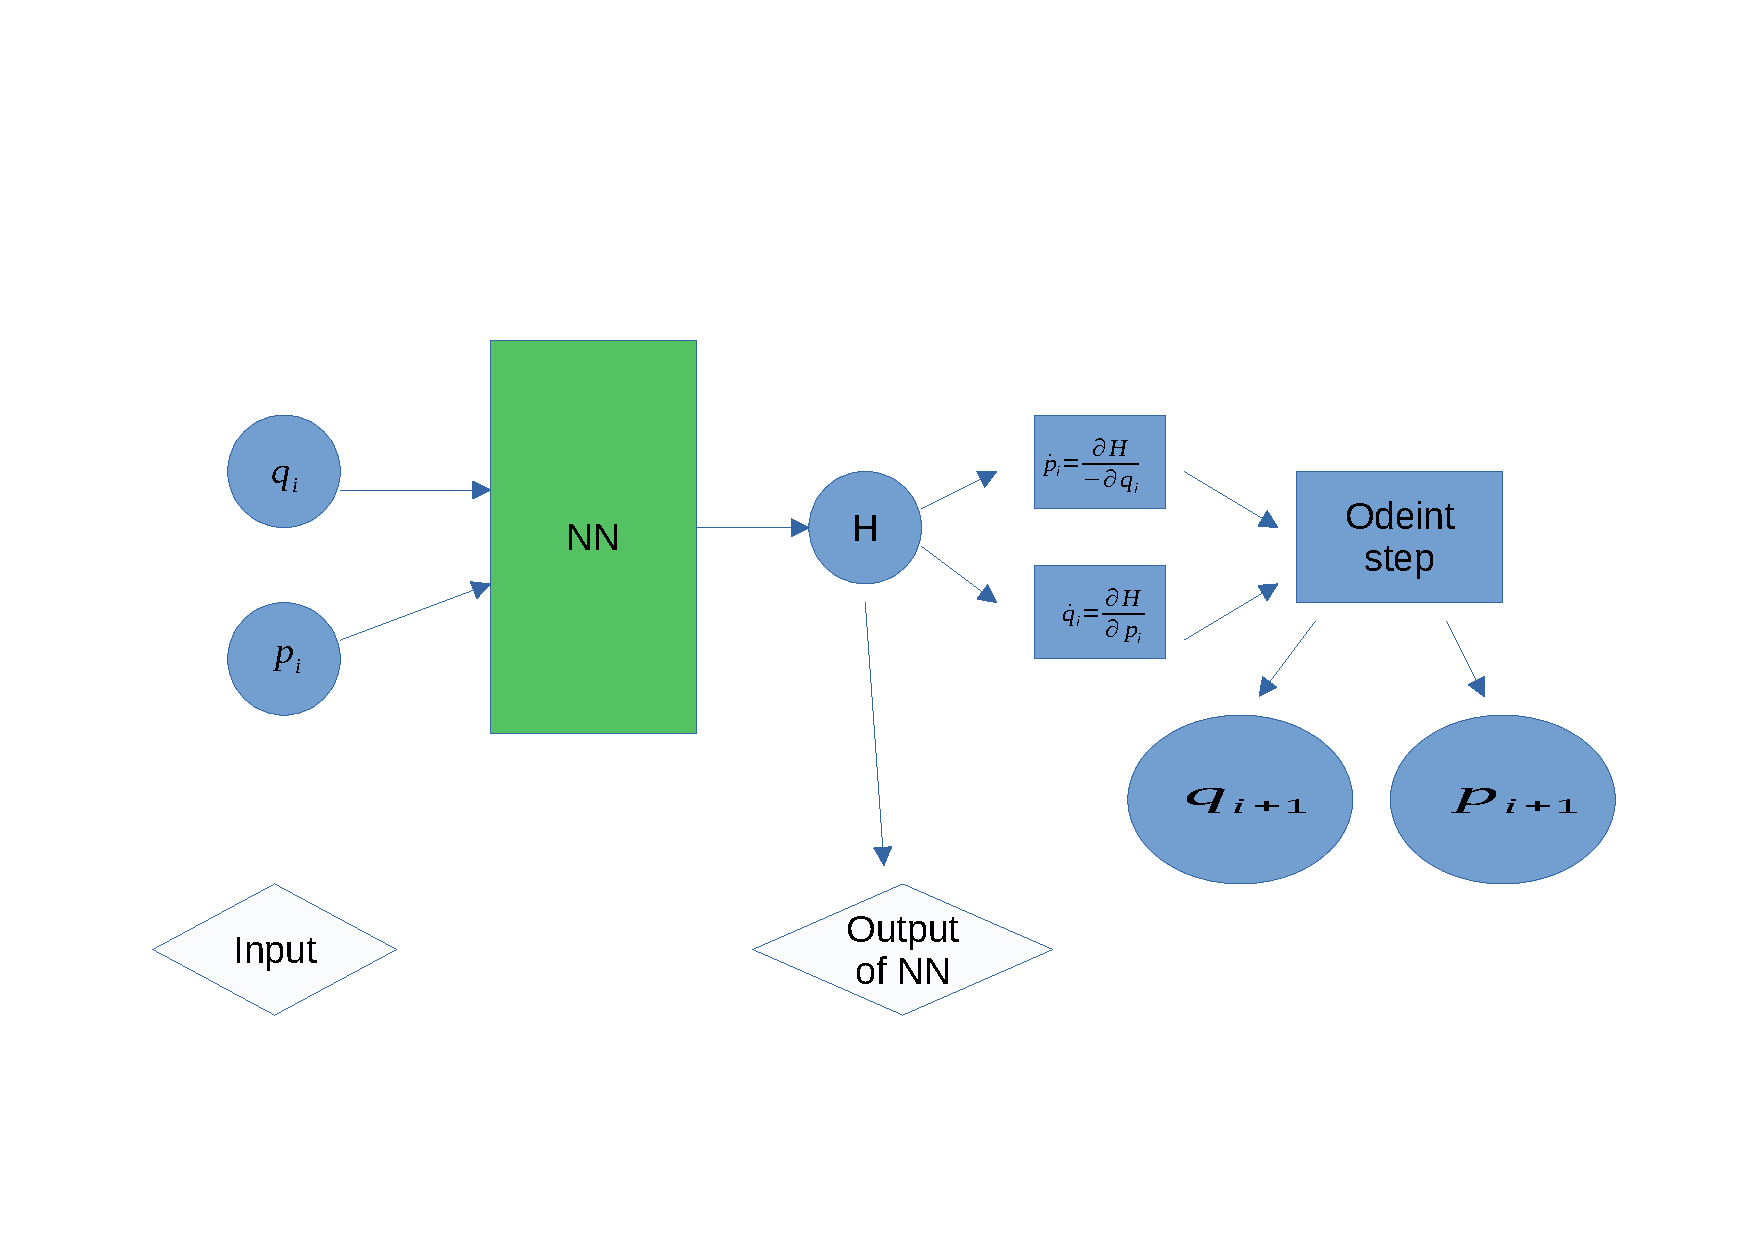
\includegraphics[width=15cm]{chapters/chapter1/hnn}
	\label{hnn}
	\caption{HNN model with integration solver step}
\end{figure}
One of such model is introduced in the \cite{} and it is called HNN. it architecture you can observe in figure \ref{hnn}.
We will make it more interesting introducing the Graph Neural Network and try to use it as a base of our architecture.\\
In this thesis we will discuss what are Hamiltonian equations and how to obtain them. In our research we stumbled upon the fact, that there are no quality datasets for training the Neural Networks which are based on physics. With this fact we brew 4 popular datasets which are based on Hamiltonian Equations of Motion.\\
Next we made new and revisit old neural architectures and test NeuralODE as new Nerual Paradigm into treaining the solutions of ODEs.\\
In the experiments we tested the capabilites of Graph Neural Networks, how do they adapt to diverse training data and their possibility to reduce or increase a degree of freedom in the training. For example how similar is the movement between 3 and 4 bodied pendulum on the same trained set of neural parameters. We hope that we will give the insight in those topics.    








%% related works, philosophy, motivations, my contributions

\chapter{Background}\label{background}
%In this chapter we will discuss main topics from Classical Mechanics and refresh out knowledge about common neural network architectures. This will be needed to understand the working of our Physics informed networks in chapter Methods.
In this chapter, we revisit some of the important concepts from Classical Mechanics and further develop an understanding of common neural network architectures. This is a critical foundation which will be required to understand how Physics-Informed Neural Networks work, as discussed in greater detail in the Methods chapter. 
\section{Classical Mechanics}\label{cs}
%The classical physics are most important science to understand the laws which govern how mass object behaves in our reality. Such science is called the Classical Mechanics. It tend to describe how the mass moves in space. Simply the movement manifests through forces applied on the matter. Sir Isaac Newton for this observed phenomena gave a laws which masses should obey  \cite{ClassPhy}
Classical Physics presents the basics for understanding the laws presiding over the behavior of objects with mass in our physical reality. This aspect of the science of Classical Mechanics describes how mass moves in space: motion is the result of forces applied to matter. Moving on, Sir Isaac Newton did develop laws that describe and predict the behavior of such objects, which today are called the Newton's Laws of Motion.\cite{ClassPhy}
\begin{itemize}
	\item Newton's 1st law: Unless acted on by an outside force the natural motion of an object is constant velocity
	\item Newton’s 2nd law: The effect of an applied force $\mathbf{F}$ upon an object of mass
	m is to induce an acceleration $\mathbf{a}$ such that $$\mathbf{F}=m\mathbf{a}$$
	If mass is constant we can introduce momentum $\mathbf{p}$.
	$$\mathbf{F}=\frac{d\mathbf{p}}{dt}$$ \\
	Derivation of the momentum in time t is a force. 
	With this equation we can obtain momentum as $$\mathbf{p}=m\mathbf{v}$$ where $\mathbf{v}$ is velocity.
	\item Newton’s 3rd law: If an object applies a force $\mathbf{F}$ on a second object, then the second object applies an equal and opposite force $-\mathbf{F}$ on the first object.\\
	In the physics it is most famous law and it is often referenced as  \textit{actio = reactio} from latin.
\end{itemize}
One of the simplest systems that adheres to these laws is the harmonic oscillator.
\subsection{Harmonic Oscilator}
Harmonic Oscilator is  system  in classical physics which describes the situation where body is displaced from equilibirium position and it experience the restoring force $\mathbf{F}$ proportional to its displacement. This system is described with Ordinary Differential Equation of second order : 
\begin{equation}
	m\ddot{\mathbf{x}}(t) = -k\mathbf{x}(t) \texttt{,   } \mathbf{x}(0)= \mathbf{x}_0
\end{equation}
We will consider this system as one dimensional $\mathbf{x}= x$
in which the harmonic motion is along straight line, the motion is said to be simple harmonic motion \cite{osci}. To show the simple harmonic motion let us solve the equation.\\
First we will build the the linear system of equations to get the first order ordinary differential equation in form: \begin{equation}
	\ddot{\mathbf{z}}= \mathbf{A}\mathbf{z} + \mathbf{b}.
\end{equation}
We are beginning with parameter $z$:
\begin{eqnarray}
	z_1 &=& x\\
	z_2 &=& \dot{x}\\
	\dot{z}_1 &=& \dot{x} = z_2\\
	\dot{z}_2 &=& \ddot{x} = -\frac{k}{m}z_1 
\end{eqnarray}
With this we got:
\begin{equation}
	\begin{bmatrix}
		\dot{z_1}\\
		\dot{z_2}\\
	\end{bmatrix} = \begin{bmatrix}
	0 & 1\\
	-\frac{k}{m} & 0\\
	\end{bmatrix}
	\begin{bmatrix}
		z_1\\
		z_2\\
	\end{bmatrix}
\end{equation}
We got differential ordinary equation which is homogeneous ($\mathbf{b}=0$). To solve this Problem we need to refresh the knowledge of solving the ODEs 

\subsection{Analytical solution of Ordinary Differential Equations}
A Differential Ordinary Equation of the first order is defined as:
\begin{equation}
\label{eq:diff}
\dot{\mathbf{z}}= \mathbf{A}\mathbf{z} + \mathbf{b}u \texttt{, }\mathbf{z}(0) = \mathbf{z}_0
\end{equation}
Before we show analytical solution of mentioned linear system, let us solve first the simplest case:
 
\begin{equation}
	\dot{z}(t)= az(t) + bu \texttt{, }z(0) = z_0
\end{equation}
Every solution of ODE has homogeneous $z_{hom}$ and particular solution $z_{par}$
\begin{equation}
	z(t) = z_{hom} + z_{par}.
\end{equation}
When we calculate de homogeneous solution we set $b=0$ and we precede with simple integration.
\begin{equation}
	\int\frac{dz}{z} = \int adt
\end{equation}
\begin{equation}
	\boxed{z_{hom}= c\exp(at)}
\end{equation}
To find particular solution we will create it with variation of the constants method.\\
We define:
\begin{equation}
	z_{part}= c(t)\exp(at)
\end{equation}
and we will put it in the differential equation
\begin{eqnarray}
	\dot{z}_{part}(t)&=& az_{part}(t) + bu(t),\\
	a\exp(at)c(t)+ \exp(at)\dot{c}(t)&=& a\exp(at)c(t) + bu(t),\\
	\dot{c}(t) &=& \exp(-at)bu(t).
\end{eqnarray}
After integration of $\dot{c}$ we get:
\begin{equation}
	\boxed{z_{part}= c(0)\exp(at) + \int^t_0 \exp(at-\tau)bu(\tau)d\tau}
\end{equation}
With inclusion of the Initial condition $z(0) = z_0$ we get final form of the solution \\
\begin{equation}
	\boxed{z= \underbrace{z_0\exp(at)}_\text{homogeneous} + \underbrace{\int^t_0 \exp(a(t-\tau))bu(\tau)d\tau}_\text{particular} }.
\end{equation}
Let so go back and solve the equation \ref{eq:diff}.\\
Obtaining the solution goes similar to simple case but it is vectorized.\\
The solution is made by homogeneous and particular solution as above.\\
\begin{equation}´
	\mathbf{z}=\mathbf{z}_{hom} + \mathbf{z}_{in}
\end{equation} 
Lets assume from the example what we have done previously that our homogeneous solution is defined as:
\begin{equation}
	\mathbf{z}_{hom}=\exp(\mathbf{A}t)\mathbf{c}
\end{equation}
This is easy to prove trough Taylor series of the $\exp(\mathbf{A}t)$.
\begin{equation}
	\exp(\mathbf{A}t) = \sum^{\infty}_{i=0}\frac{(\mathbf{A}t)î}{i!} = \mathbf{I}+ \mathbf{A}t+\mathbf{A}^2 \frac{t^2}{2!}+ \mathbf{A}^3 \frac{t^3}{3!} + \mathcal{O}(t^4)
\end{equation}
\begin{eqnarray}
	\frac{d\exp(\mathbf{A}t)}{dt} &=& \mathbf{A}+\mathbf{A}^2 t+ \mathbf{A}^3 \frac{t^2}{3!} + \mathcal{O}(t^3)=\\
	&&\mathbf{A}\left(\mathbf{I}+ \mathbf{A}t+\mathbf{A}^2 \frac{t^2}{2!}\right) + \mathcal{O}(t^3)\\
	&&\mathbf{A}\exp(\mathbf{A}t)
\end{eqnarray}
Lets put it in the equation
\begin{eqnarray}
	\dot{\mathbf{z}}_{hom}&=& \frac{d\exp(\mathbf{A}t)}{dt}\mathbf{c} =\\
	&&\mathbf{A}\exp(\mathbf{A}t)\mathbf{c} =\\
	&& \mathbf{A}\mathbf{z}_{hom}
\end{eqnarray}
and the homogeneous solution
\begin{equation}
	\boxed{
	\mathbf{z}_{hom} = \exp(\mathbf{A}t)\mathbf{c}}
\end{equation}
fulfills the equation.\\
With the variation of the constant method we obtain the particular solution:
\begin{equation}
\exp(\mathbf{A}t)\mathbf{c}(0)+ \int^t_0 \exp(\mathbf{A}(t-\tau))\mathbf{b}u(\tau)d\tau
\end{equation}
With inclusion of the initial condition $z(0) = z_0$ we get final form of the solution \\
\begin{equation}
	\boxed{\mathbf{z}= \underbrace{\exp(\mathbf{A}t)\mathbf{x}_0}_\text{homogeneous} + \underbrace{\int^t_0 \exp(\mathbf{A}(t-\tau))bu(\tau)d\tau}_\text{particular}}.
\end{equation}\\
In our work the most important part is homogeneous solution and to obtain that we should use standard practice to solving it.\\
\begin{itemize}
	\item Find eigenvalues and eigenvectors- Every matrix with full rank is diagonalizable 
	\begin{eqnarray}
		\mathbf{A} &=& \mathbf{V}\mathbf{D}\mathbf{V}^{-1}\\
		\mathbf{D} &=& \texttt{diag}(\{\lambda_1,...,\lambda_i,...\lambda_n\}) \text{    Eigenvalues}\\`
		\mathbf{V} &=& \left[\mathbf{v}_1|...|\mathbf{v}_i|...|\mathbf{v}_n\right] \text{    Eigenvectors}
	\end{eqnarray}
	It is easily obtained through characteristic polynomial $p(\lambda) =\det(\mathbf{A}-\mathbf{I}\lambda)=0$
	
	\item To find general solution we need to transform the $\dot{\mathbf{z}}= \mathbf{A}\mathbf{z}$
	\begin{eqnarray}
		\dot{\mathbf{z}} &=& \mathbf{V}\mathbf{D}\mathbf{V}^{-1}\mathbf{z}\\
		\underbrace{\mathbf{V}^{-1}\dot{\mathbf{z}}}_\text{} &=& \mathbf{D}\underbrace{\mathbf{V}^{-1}{\mathbf{z}}}_\text{}\\
		\dot{\boldsymbol{\Theta}}&=&\mathbf{D}\boldsymbol{\Theta}
	\end{eqnarray}
	This system is now trivial to solve.
	\item Set it in general solution $\Theta_i=c_i\exp(\lambda_i t)$ 
	In case of repeated eigenvalue we should use $\Theta_i=c_i \frac{t^r}{r!} \exp(\lambda_i t)$ where $r$ is number of repetitions.
	It will came up from the eigenvectors. 
	\item back-substitute $\mathbf{z}$
	\begin{eqnarray}
		\mathbf{z} &=& \mathbf{V}\boldsymbol{\Theta} =\sum^n_{i=1}\mathbf{v}_i\Theta_i\\
		\mathbf{z} &=& \sum^n_{i=1} \mathbf{v}_i\underbrace{c_i\exp(\lambda_i t)}_\text{\Theta}
	\end{eqnarray}
	\item apply initial conditions
	\begin{eqnarray}
	\mathbf{z}(0) = \sum^n_{i=1} \mathbf{v}_i c_i = \mathbf{V}\mathbf{c} &=&\mathbf{z}_0\\
	\mathbf{c} &=&\mathbf{V}^{-1}\mathbf{z}_0
    \end{eqnarray}
	
\end{itemize}

In this procedure we obtained the homogeneous solution. The particular solution is in some cases trivial but in some not solvable analytically due to $\mathbf{b}u(t)$. It is possible that it is nonlinear function. 
In those cases we use numerical methods to obtain the solutions.

\subsection{Numerical solution of Ordinary Differential Equations}
For every every ODE there is solution, sometimes there is no analytical solution but we can obtain numerical one trough numerical integrators. 
Still numerical solutions are only approximations of the analytical solution. Due to their stability we differ two categories of one-step methods and that are explicit and implicit methods.\\
\begin{itemize}
	\item explicit methods are trivial to calculate because the next step is dependent only on the previous step:
	\begin{equation}
		x(t_{i+1}) = x(t_i) + h\Phi(x(t_i)),t_i)
	\end{equation}
	\item implicit methods are chalenging because the next step is dependent on itself.
	\begin{equation}
		x(t_{i+1}) = x(t_i) + h\Phi(x(t_{i+1})),t_{i+1})
	\end{equation}
To obtain the step it is needed to know  function $\Phi$ and solving a next step trough some method like  for example Einstein-Raphson method. 
\end{itemize}
To assure the stability and correctness of the methods we need to set some properties.
The properties that the every one-step method should have, are Consistency and Convergence.\\

The Consistency are proven over local discretisation error.
Let say that for $(x,y)\in  \mu = \mu(\eta)$ is a solution for the ODE $\mu^{'} = f(\eta,\mu), \mu(x)=y$,then the discretisation error is
\begin{equation}
	le(x,y;h) = \mu(x+h)-\mu{x}-h\Phi(x,y;h)
\end{equation}
and discretisation error per step
\begin{equation}
	\Delta(x,y;h)=\frac{le(x,y;h)}{h}. 
\end{equation}
A one-step method is consistent if
\begin{equation}
	\lim_{h\rightarrow 0} \Delta(x,y;h) = 0.
\end{equation}
For the method to be convergent need to be consistent. The general definition of convergency is
\begin{equation}
\lim_{h\rightarrow 0} \Phi(x,y;h) = f(x,y)
\end{equation}
To prove this we should look for the consistency and convergency rank.
\begin{itemize}
	\item Consistency rank $p$\begin{equation}
		||\Delta(x,y;h)||\leq Kh^p
	\end{equation}
\item Convergency rank $p$
\begin{eqnarray}
	E(h) &=& \max_{j=0,1,...N}||y_j-y(x_j)||\text{ global discretisation error }\\
	\lim_{h\rightarrow 0}E(h) &=& 0 \text{ Convergence}\\
	E(h) &\leq&  Kh^p
\end{eqnarray}



\end{itemize} 
This properties are highly important to know because we will use for the experiments mostly the Runga-Kutta methods which are based on those properties.\\
Most important for us are
\begin{itemize}
	\item Euler method
		\begin{equation}
			x_{i+1} = x_i + hf(x_i,t_i)
		\end{equation}
	\item Runge-Kutta 4 Method(RK4)
		\begin{eqnarray}
			K_1 &=& f(x_i,t_i)\\
			K_2 &=& f(x_i + \frac{h}{2}K_1,t_i +\frac{h}{2})\\
			K_3 &=& f(x_i + \frac{h}{2}K_2,t_i+\frac{h}{2})\\
			K_4 &=& f(x_i + hK_3,t_i +h)\\
			x_{i+1} &=& x_i + \frac{h}{6}(K_1 + 2K_2 +2K_3 +K_4)
		\end{eqnarray}	
	\item Dormand- Prince method is most accurate method for obtaining he solutions of ODEs\cite{dopri5}.
	It is widely used in experiments.\\
		
\end{itemize}
\subsection{Solving the harmonic oscilator}
In one of the previous subsections we obtained the first order ODE for harmonic oscilator and we described how it should be solved.
\begin{equation}
	\begin{bmatrix}
		\dot{z_1}\\
		\dot{z_2}\\
	\end{bmatrix} = \begin{bmatrix}
		0 & 1\\
		-\frac{k}{m} & 0\\
	\end{bmatrix}
	\begin{bmatrix}
		z_1\\
		z_2\\
	\end{bmatrix}\text{   , }\mathbf{z}_0 = \begin{bmatrix}
x_0\\
v_0\\
\end{bmatrix}
\end{equation}
Through the system Matrix $A = \begin{bmatrix}
	0 & 1\\
	-\frac{k}{m} & 0\\
\end{bmatrix}$ we got complex eigenvalues, which are $\lambda_1 = i\sqrt{\frac{k}{m}}$ and $\lambda_2 = -i\sqrt{\frac{k}{m}}$.\\
General solution of this problem is
\begin{equation}
	z_1 = x = c_1\exp(i\sqrt{\frac{k}{m}}t) + c_2\exp(i\sqrt{-\frac{k}{m}}t)
\end{equation}
With applying of the euler formula:
\begin{equation}
	\exp(iat)=\cos(at) + i\sin(at)
\end{equation}
We get simplified solution
\begin{eqnarray}
	z_1 &= x =& (c_1+c_2)\cos\left(\sqrt{\frac{k}{m}}t\right) + (c_1-c_2)i\sin\left(\sqrt{\frac{k}{m}}t\right)\\
	z_2 &= \dot{x} =& -(c_1+c_2)\sqrt{\frac{k}{m}}\sin\left(\sqrt{\frac{k}{m}}t\right)+(c_1-c_2)\sqrt{\frac{k}{m}}i\cos\left(\sqrt{\frac{k}{m}}t\right).
\end{eqnarray}
Now we can apply initial conditions
\begin{eqnarray}
x(0)=x_0 = c_1 + c_2,\\
\dot{x}(0)=v_0 = i(c_1-c_2).
\end{eqnarray}
The velocity in our cases is an real number which we can assume that constants $c_1$ and $c_2$ are equal. 
This simplifies our equations  and we can substitute $x_0 = c_1 +c_2$
\begin{eqnarray}
	z_1 &= x =& x_0\cos\left(\sqrt{\frac{k}{m}}t\right),\\
	z_2 &= \dot{x} =& -x_0\sqrt{\frac{k}{m}}\sin\left(\sqrt{\frac{k}{m}}t\right)
\end{eqnarray}
The is harmonic at we can se that clearly because it is periodic and we can read an angle velocity of periodic movement $\omega = \sqrt{\frac{k}{m}}$,
\begin{eqnarray}
	z_1 &= x =& x_0\cos\left(\omega t\right)\\
	z_2 &= \dot{x} =& -x_0\omega\sin\left(\omega t\right)
\end{eqnarray}
\subsection{Langrange and Hamiltonian Equations}
In robotics, research and model creation of the robot models are not only one-bodied system. Mostly they are are rigid-body systems like a manipulator which has N degrees of freedom. Every of the joints and links have own properties like mass, friction, etc.\\
The Kinematic of the model and irreversibility is possible to calculate with mathematic methods. Kinematic is just establishing the function which with correct input like angles of joints $q$ give as an output in form of target position of the endeffector. This easy easy to establish with Denavit–Hartenberg convention.  On the other hand determining Dynamics is not trivial task. The Dynamic creates trajectory which is in form of ODE.\\
There is one most popular method to solve and establish Dynamics of the model and that are Lagrange Equations.
\subsubsection{Lagrange Equations}
Langrage Equations are derived from D’Alambert Principle which is an alternative to the Newton's second law\cite{ClassPhy}:
\begin{equation}
	\mathbf{F} = m\mathbf{a}
\end{equation}   
In the case of the rigid body:
\begin{equation}
	\mathbf{F}_i = \sum_i{m_i \mathbf{a}_i}
\end{equation}
To derive Lagrangian Equations which describes dynamics we need first to define constraints. Let us define homonomic constraints.
For $N$ bodies B = $\{\mathbf{r}_1,...,\mathbf{r}_i,...,\mathbf{r}_N\}\text{ ; } \mathbf{r}_i=\mathbf{r}_i(q_1,...,q_i,...,q_n, t)$
\begin{equation}
	\boxed{G_k(\mathbf{r}_1,..,\mathbf{r}_i,..,\mathbf{r}_n,t)=0\text{ for}k=1,..M}
\end{equation}
Where the $q_i$ are generalized coordinates and the
parameters are also constrained as $3\cdot M\cdot N = n$.\\
In case of two dimensional N-Pendulum some of that constraints would look like:
\begin{equation}
	G_i := \left|\left|\mathbf{r}_i - \mathbf{r}_{i+1}\right|\right| - d_i = 0
\end{equation}
This says that the distance between two neighboring joints are constant.
holonomic constraint defines the relation between bodies $\r_i$ on some configuration space $\mathcal{A}$.
Lets go back to the second newton law and lets apply holonomic constraint. With holonomic constraint we can spilt $\mathbf{F}$ on constraint force $\mathbf{F}^c$ and apllied force $\mathbf{F}^a$.
\begin{equation}
	\mathbf{F} =\mathbf{F}^c + \mathbf{F}^a
\end{equation}
Now we will apply virutal Work principle, which comes from orthogonality of virtual displacement and constraint forces \cite{ortho}
\begin{equation}
	\boxed{\sum_i{\mathbf{F}_i^c \cdot \underbrace{\delta \mathbf{r}_i}=0}_\text{virtual displacement}}
\end{equation}
to the constrained Newton's second law we get following formula which is D'Alambert principle\cite{dalam}:
\begin{eqnarray}
	 \mathbf{F}^c_i &=& \mathbf{F}_i- \mathbf{F}^a_i\\
	 \sum_i{\mathbf{F}_i^c \cdot \delta \mathbf{r}_i} &=& \sum_i{(\mathbf{F}_i- \mathbf{F}^a_i) \cdot \delta \mathbf{r}_i}\\
	 \sum_i{(\mathbf{F}_i- m_i\ddot{\mathbf{r}}_i) \cdot \delta \mathbf{r}_i}&=&0\text{    D'Alambert Principle}
\end{eqnarray}\\
If we need virtual displacement for the generalized coordinates:
\begin{equation}
	\delta\mathbf{r}_i = \sum_j^n{\frac{\partial\mathbf{r}_i}{\partial q_j}\cdot \delta q_j}
\end{equation}
Now we can derive Langrange Equations applying last equation to D'Alambert principle:
\begin{eqnarray*}
\sum_i^N{\mathbf{F}_i \cdot \delta \mathbf{r}_i} &=& \\ \sum_i^N{\mathbf{F}_i\sum_j^n{\frac{\partial\mathbf{r}_i}{\partial q_j}\cdot \delta q_j}}&=&\\
\sum_j^n{\delta q_j\underbrace{\sum_i^N{\mathbf{F}_i}\frac{\partial\mathbf{r}_i}{\partial q_j}}_\text{$Q_j$}}&=&\boxed{\sum_j^n{\delta q_j\cdot Q_j}}\\
\sum_i^N{m_i\ddot{\mathbf{r}}_i \cdot \delta \mathbf{r}_i}&=&\\
\sum_i^N{m_i\ddot{\mathbf{r}}_i \sum_j^n{\frac{\partial\mathbf{r}_i}{\partial q_j}\cdot \delta q_j}}&=&
\sum_j^n{\delta q_j\sum_i^N{m_i\ddot{\mathbf{r}}_i\frac{\partial\mathbf{r}_i}{\partial q_j}}}\\
\text{with substitution of: } \frac{\partial\dot{\mathbf{r}_i}}{\partial \dot{q_j}} &=& \frac{\partial}{\partial \dot{q_j}}\left(\frac{d\mathbf{r}_i}{dt} + \sum^N_i{\frac{\partial \mathbf{r_i}}{q_j}\dot{q_j}}\right) = \frac{\partial \mathbf{r_i}}{q_j}\\
\sum_i^N{m_i\ddot{\mathbf{r}}_i \sum_j^n{\frac{\partial\mathbf{r}_i}{\partial q_j}\cdot \delta q_j}}&=&
\sum_j^n{\delta q_j\sum_i^N{m_i\ddot{\mathbf{r}}_i\frac{\partial\dot{\mathbf{r}_i}}{\partial \dot{q_j}}}}\\
\text{with: }\sum_i^N{\frac{d}{dt}m_i\dot{\mathbf{r}}_i\frac{\partial\dot{\mathbf{r}_i}}{\partial \dot{q_j}}} &=& \sum_i^N{m_i\ddot{\mathbf{r}}_i\frac{\partial\dot{\mathbf{r}_i}}{\partial \dot{q_j}}+m_i\dot{\mathbf{r}_i}\frac{d}{dt}\frac{\partial \mathbf{r}_i}{\partial q_j}}\\
\sum_j^n{\delta q_j\sum_i^N{m_i\ddot{\mathbf{r}}_i\frac{\partial\mathbf{r}_i}{\partial \dot{q_j}}}} &=& \sum_j^n{\delta q_j\sum_i^N{\frac{d}{dt}\left(m_i\dot{\mathbf{r}_i}\frac{\partial\dot{\mathbf{r}_i}}{\partial \dot{q}}\right)-m_i\dot{\mathbf{r}_i}\frac{\partial\dot{\mathbf{r}_i}}{\partial q}}}\\
\end{eqnarray*}
We get this equation
\begin{equation}
\boxed{\sum_i^N{m_i\ddot{\mathbf{r}}_i \cdot \delta \mathbf{r}_i} =\sum_j^n{\delta q_j\left[\frac{d}{dt}\frac{\partial}{\partial \dot{q_j}}\left(\sum_i^N\frac{1}{2}m_i\dot{\mathbf{r}_i}^2\right)-\frac{\partial}{\partial \dot{q_j}}\left(\sum_i^N\frac{1}{2}m_i\dot{\mathbf{r}_i}^2\right)\right]}}
\end{equation}
With those two made equations we can finally put it togehter in D'Alambert Principle formula:
\begin{equation}
	\sum_j^n{\delta q_j\left[\frac{d}{dt}\frac{\partial}{\partial \dot{q_j}}\left(\sum_i^N\frac{1}{2}m_i\dot{\mathbf{r}_i}^2\right)-\frac{\partial}{\partial q_j}\left(\sum_i^N\frac{1}{2}m_i\dot{\mathbf{r}_i}^2\right)- Q_j\right]} =0 
\end{equation}
This Equation is almost complete, we need to define the energies and their specifications

\begin{itemize}
	\item Kinetic Energy - Energy possessed by bodies due to their motion.\\
	The Formula for kinetic energy is
	\begin{equation}
		T(q,\dot{q}) = \sum_i^N\frac{1}{2}m_i\dot{\mathbf{r}_i}^2
	\end{equation}
	\item Potential Energy - Energy held by body becuase of its relative position to other bodies or other target.\\
	There is many types of potential energy:\\
	Pendelum - $U(q=h)=mgh$\\
	Oscilator - $U(q)=\frac{kq}{2}$ 
\end{itemize}
In the Formula $\mathbf{Q}$ is generalized force and it is created from the gradient of the potential energy and it is conservative :
\begin{equation}
	\mathbf{Q_j} =- \sum^N_i \nabla_{\mathbf{r_i}}U(q)\frac{\partial\mathbf{r_i}}{\partial q_j}= -\frac{\partial U}{\partial q_j}
\end{equation} 
Potential Energy is only dependent on position of the bodies $\frac{\partial U}{\partial \dot{q}} = 0$.\\
The Lagrange Equations for holonomic constrains and conservative force is defined as:
\begin{eqnarray}
\frac{d}{dt}\frac{\partial}{\partial \dot{q_j}}\left(T-U\right)-\frac{\partial}{\partial q_j}\left(T-U\right) =0\\
\frac{d}{dt}\frac{\partial}{\partial \dot{q_j}}\mathcal{L}-\frac{\partial}{\partial q_j}\mathcal{L} =0
\end{eqnarray}
$\mathcal{L}$ is called Lagrangian.
\subsubsection{Hamiltonian Equations}
To derive Hamiltonian Equations we need an Lagrangian $\mathcal{L}$.
We have two famous derivation of Langrangian and that are:
\begin{equation}
	\frac{\partial\mathcal{L}}{\partial \mathbf{q}} = \dot{\mathbf{p}}
\end{equation}
\begin{equation}
	\frac{\partial\mathcal{L}}{\partial \dot{\mathbf{q}}} = \mathbf{p}
\end{equation}
Through Legendre Transformation we can obtain Hamiltonian $\mathcal{H}$
\begin{equation}
	\mathcal{H}(\mathbf{q},\dot{\mathbf{q}},\mathbf{p},t) = \sum_i^N  \dot{\mathbf{q}_i} \cdot \mathbf{p}_i -\mathcal{L}(\mathbf{q},\dot{\mathbf{q}},t)
\end{equation}
With total derivation\cite{ham} we get
\begin{eqnarray}
	d\mathcal{H} &=& \sum_i^N\left[ \dot{\mathbf{q}} d\mathbf{p}_i +  \mathbf{p}_i d\dot{\mathbf{q}_i} - \frac{\partial\mathcal{L}}{\partial \mathbf{q}_i} d\mathbf{q}_i - \frac{\partial\mathcal{L}}{\partial \dot{\mathbf{q}_i}} d\dot{\mathbf{q}_i}\right] - \frac{\partial\mathcal{L}}{\partial t} dt\\ 
	&=& \sum_i^N\left[ \dot{\mathbf{q}} d\mathbf{p}_i +  \mathbf{p}_i d\dot{\mathbf{q}_i} - \dot{\mathbf{p}_i} d\mathbf{q}_i - \mathbf{p}_i d\dot{\mathbf{q}_i}\right] - \frac{\partial\mathcal{L}}{\partial t} dt\\
	&=&\sum_i^N\left[ \dot{\mathbf{q}} d\mathbf{p}_i  - \dot{\mathbf{p}_i} d\mathbf{q}_i\right] - \frac{\partial\mathcal{L}}{\partial t} dt\\
\end{eqnarray}
On the other hand we want hamiltonian which is dependent on canoical moment and generalized coordinates $\mathcal{H}=\mathcal{H}(\mathbf{q},\mathbf{p},t)$
In that case the total derivation of Hamiltonian $\mathcal{H}$ is
\begin{equation}
	d\mathcal{H} = \sum_i^N\left[\frac{\partial \mathcal{H}}{\partial \mathbf{q}_i}d\mathbf{q}_i + \frac{\partial \mathcal{H}}{\partial \mathbf{p}_i}d\mathbf{p}_i\right] + \frac{\partial\mathcal{H}}{\partial t} dt
\end{equation}
With comparing both equivalent derivations we can define the equations of motion:
\begin{equation}
	\dot{\mathbf{p}} = -\frac{\partial \mathcal{H}}{\partial \mathbf{q}}
\end{equation}
\begin{equation}
	\dot{\mathbf{q}} = \frac{\partial \mathcal{H}}{\partial \mathbf{p}}
\end{equation}
\begin{equation}
	\frac{\partial\mathcal{H}}{\partial t} = - \frac{\partial\mathcal{L}}{\partial t}
\end{equation}
Hamiltonian equations are very useful because in the case $\frac{\partial\mathcal{H}}{\partial t} = 0$ our Total Energy $\mathcal{H} = E = T + U$ is conserved and often we can derive time independent motion.
\section{Neural Network Architectures}
At the beginning of our research we experimented with feedforward networks and recurrent networks.  
\subsection{Deep forward Network - Multilayer Perceptron }
Feedforward networks like Multilayer perceptron approximates a certain function $\mathbf{f(\mathbf{x})}$. As MLP function we will show it as a mapping $\mathbf{f}(\mathbf{x}|\Theta)$.\\
The main goal of feedforward network is to fit the model so that the we get best approximation. Fit the model means to learn the parameters of the model trough optimizing procedure.\\
Multiplayer perceptron is fully connected feedforward neural network. The nodes of the MLP are often called neurons and they build a layer. A minimal MLP has three consecutive layers: which form complete bipartite graph.\\
Mathematical expression of one neuron:
\begin{equation}
	y = \sigma(\sum_i{w_i \cdot x_i} + b) 
\end{equation}
Mathematical expression of the feedforward layer network:
\begin{equation}
	\mathbf{h}^{(k+1)} =\sigma\left(\mathbf{W}^{(k)}\mathbf{h}^{(k)} + \mathbf{b}^{(k)}\right)
\end{equation} and we can see graphical representation in \ref{mlp}
In this equation $\sigma$ is called activation function, 
$\mathbf{W}$ as weights and $\mathbf{b}$ as bias which are our parameters $\Theta =\{\mathbf{W},\mathbf{b}\}$.\\
\begin{figure}[h!]
	\centering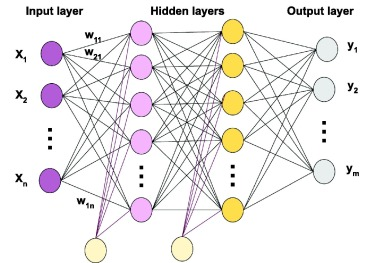
\includegraphics[width=8cm]{chapters/chapter2/mlp}
	\caption{Multilayer perceptron\cite{mlppic}}
	\label{mlp}
\end{figure}
The activation function in the network introduces non linearity to improve approximation capability.\\




\subsection{Recurrent Neural Networks}
Reccurent Neural Networks are very interesting concept of Neural Network architecture. It is mostly used for speech recognition but for a time series\cite{mlprnn}.\\
Architecture of this Neural Network depends on which data we work.
There is three types which we can use\cite{rnntypes}:
\begin{itemize}
	\item many to many\\
	This type is used for speech recognition we use a dataset which has sentences and it outputs some values which could be understood from other model. Fo example translation or video captioning
	\item one to many\\
	used for the time series data from one input we can create recurrence that represent a time point with new output. From one input we get more outputs. time-series can be for example music generation.
	\item many to one\\
	from many outputs we get only one output. This is very good model for example spam detection
\end{itemize}
Let say that we have a sequence $S = \{\mathbf{x}^0,\mathbf{x}^1,...,\mathbf{x}î,..\mathbf{x}^n\}$. the first element $\mathbf{h}^0$ will be initialized as 0.
The architecture of the RNN-cell\cite{rnn} described in mathematical formulation 
\begin{eqnarray*}
	\mathbf{h}^{(i)} &=& \sigma(\mathbf{W}_{hh} \cdot \mathbf{h}^{(i-1)} + \mathbf{W}_{hx}\mathbf{x}^{(i-1)} + \mathbf{b}_h)\\
	\mathbf{y}^{(i)} &=& \sigma(W_{yh}\cdot \mathbf{h}^{(i)} + \mathbf{b}_y)
\end{eqnarray*} and graphical appearance is shown in \ref{rnn}
\begin{figure}[h!]
	\centering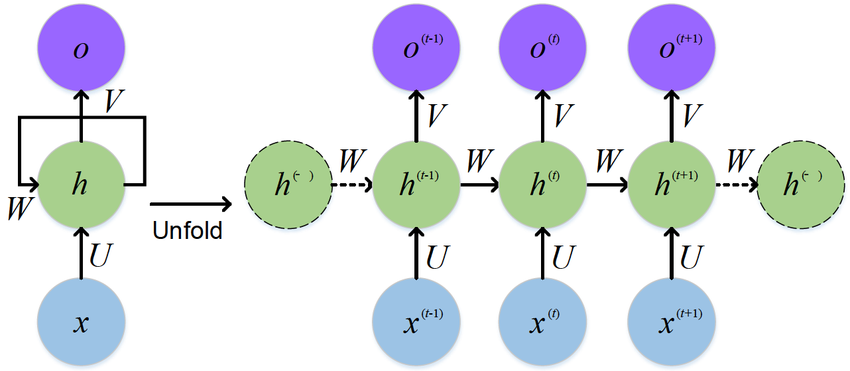
\includegraphics[width=8cm]{chapters/chapter2/rnn}
	\caption{Recurrent neural unit(many to many)\cite{rnn_picture}}
	\label{rnn}
\end{figure}

There is similar and better model then RNN and that is Gated Recurrent Unit called GRU.
We use it in same way as RNN but it his own unique architecture\cite{gru}:
\begin{eqnarray}
	r_t &=& \sigma(W_{ir} x_t + b_{ir} + W_{hr} h_{(t-1)} + b_{hr}) \\
	z_t &=& \sigma(W_{iz} x_t + b_{iz} + W_{hz} h_{(t-1)} + b_{hz}) \\
	n_t &=& \tanh(W_{in} x_t + b_{in} + r_t \odot (W_{hn} h_{(t-1)}+ b_{hn})) \\
	h_t &=& (1 - z_t) \odot n_t + z_t \odot h_{(t-1)}
\end{eqnarray} and we can see it in plot \ref{gru}
\begin{figure}[h!]
	\centering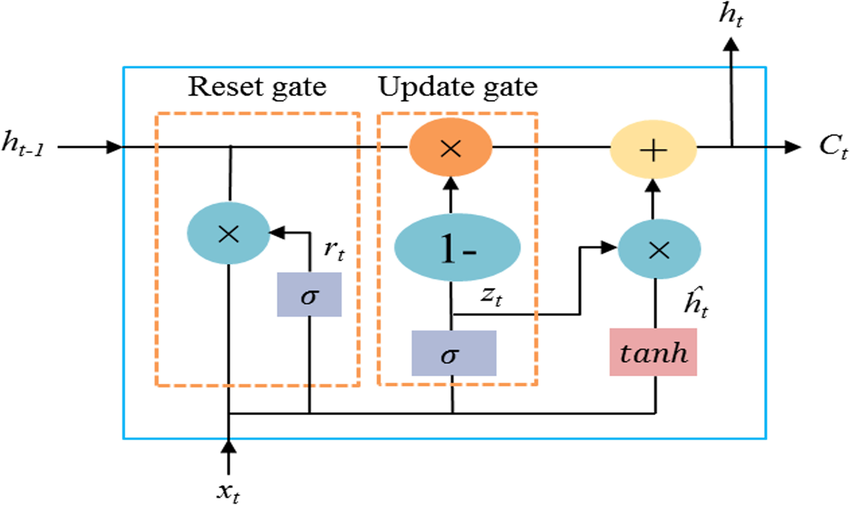
\includegraphics[width=8cm]{chapters/chapter2/gru}
	\caption{Gated recurrent unit\cite{gru_picture}}
	\label{gnn}
\end{figure}
The GRU unit is specific because it has reset gate $r_i$ and update gate $u_i$. Such architecture give better performance then at simple RNN.

\subsection{Activation functions and Loss functions}
In every neural architecture there is a activation function.
Most used activation functions are:
\begin{itemize}
	\item ReLU\\
	\begin{equation}
		\text{ReLU}(x) = max(x,0)
	\end{equation}
	This function passes only positive values.\\
	\begin{figure}[h!]
		\centering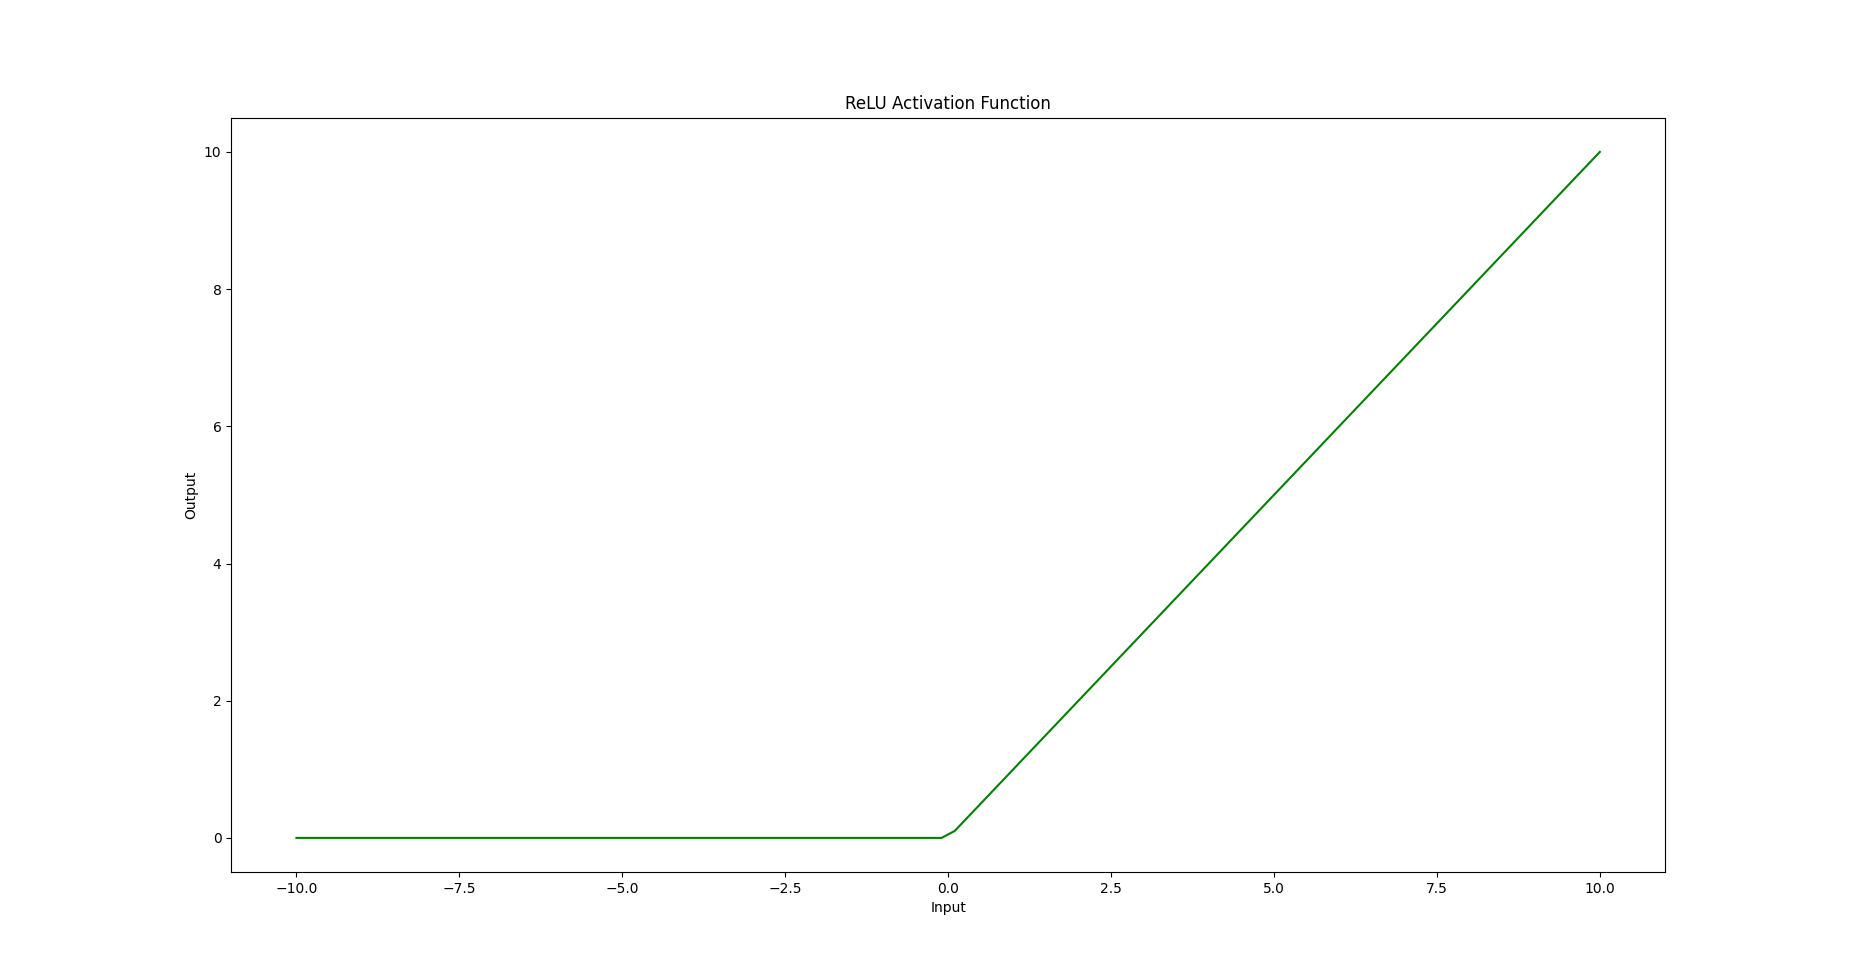
\includegraphics[width=8cm]{chapters/chapter2/relu}
		\caption{ReLU activation}
		\label{relu}
	\end{figure}
	\item tanH - It gives an output $y \in [-1,1]$\\
	\begin{figure}[h!]
		\centering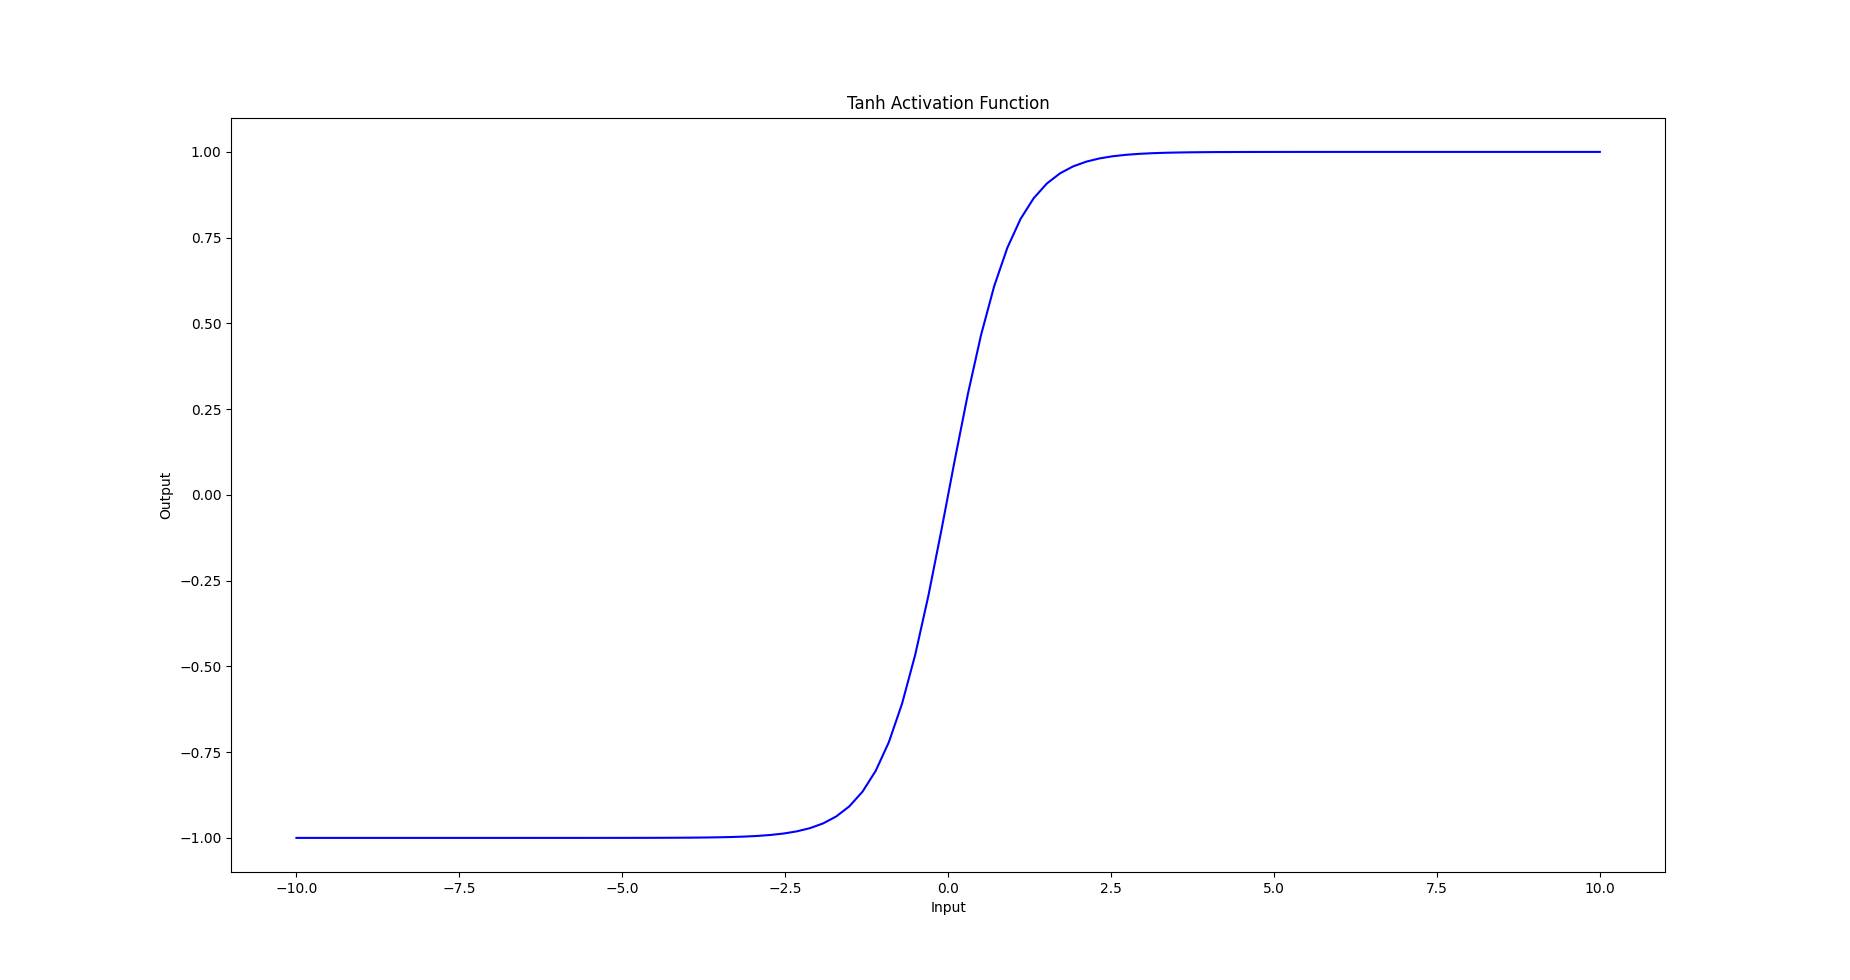
\includegraphics[width=8cm]{chapters/chapter2/tanh}
		\caption{Tanh activation}
		\label{tanh}
	\end{figure}
\end{itemize} 

Output layer has no activation function. it is connected to the loss function. The most used loss functions are:
\begin{itemize}
	\item Mean Absolute Error(MAE)
	\begin{equation}
		\text{MAE}(y,\hat{y}) = \frac{1}{N}\sum^N_i \left|y_i-\hat{y}_i\right|
	\end{equation}
	
	\item Mean Squared Error(MSE)
	\begin{equation}
		\text{MSE}(y,\hat{y}) = \frac{1}{N}\sum^N_i \left(y_i-\hat{y}_i\right)^2
	\end{equation}
	
	\item HuberLoss
	\begin{equation}
		\text{HuberLoss}(y,\hat{y};\delta) = \left\{\begin{matrix}
			\frac{1}{2}(y - \hat{y})^{2} & if \left | (y - \hat{y})  \right | < \delta\\
			\delta ((y - \hat{y}) - \frac1 2 \delta) & otherwise
		\end{matrix}\right.
	\end{equation}
	
\end{itemize}.

\subsection{Optimizers}
To do backpropagation we need an optimizer to update our learnable parameters. The easiest optimizer is stochastic gradient descent.
\begin{equation}
	\mathbf{W}^{(i+1)} =\mathbf{W}^{(i)}-\mu \frac{\partial Loss(z)}{\partial \mathbf{W}^{(i)}}
\end{equation}
There are more better one and for our use case we will use AdamW\cite{adamW}.

\subsection{Backpropagation of Neural Models}
After forward pass and calculated loss, we need to do just next steps Backward pass and optimization step.\\In backward pass we are computing the gradients of our learnable parameters to use it for the optimization of the model.\\
For example we will use stochstic gradient descent(SGD)
\begin{eqnarray}
	\mathbf{W}_{i+1} = \mathbf{W}_i - \gamma\cdot \frac{\partial Loss(z)}{\partial \mathbf{W}_i }\\
	\mathbf{b}_{i+1} = \mathbf{b}_i - \gamma\cdot \frac{\partial Loss(z)}{\partial \mathbf{b}_i }
\end{eqnarray} where $\gamma$ is a learning rate and one layered MLP
without bias $\mathbf{b}$.
\begin{eqnarray}
	\mathbf{z}_1 = \mathbf{W_0}\mathbf{y_0}\\ 
	\mathbf{y}_1 = \sigma(\mathbf{z}_1)\\
	\text{Loss}(y_1,\hat{y}) = \text{MSE}(y_1,\hat{y})
\end{eqnarray}
The obtaining the gradients of the weights is called backpropagation because for its calculation we need to apply chain rule for derivation.
\begin{equation}
\frac{\partial Loss(z)}{\partial \mathbf{W}_0}= \frac{\partial Loss(z)}{\partial \mathbf{y}_1} \cdot\frac{\partial \mathbf{y}_1}{\partial \mathbf{z}_1}\cdot	\frac{\partial \mathbf{z}_1}{\partial \mathbf{W}_0}
\end{equation}
Recurrent neural networks often fall as a victim of gradient vanishing or gradient exploding. In this manner the models doesn’t learn because the derivations calculated through backpropogation are to small or to big. It is important that gradients slowly decrease trough learning that whole model can generalize the data.

\chapter{Methods}
After previous chapters we should achieve basic understanding of neural network models and physics. With this knowledge we will introduce the methods which are capable to learn from dataset which are created trough dynamics of the systems. 
\section{New paradigm - NeuralODE}
Neural ODE is very interesting and important concept for solving the Ordinary Differential Equations and training the neural networks with trajectory data.\\
The default situation is described as:
\begin{equation}
	\dot{\mathbf{x}}=\mathbf{f}(\mathbf{x},t|\Theta)
\end{equation}
Where $\mathbf{f}(\mathbf{x},t|\Theta) $ represents the multilayer perception which creates vector field.
This method has it history from residual networks where their feed-forward network looks like euler step
\begin{equation}
	\mathbf{h}^{(i+1)} = \mathbf{h}^{(i)} + \mathbf{f}(\mathbf{h}^{(i)}|\Theta)
\end{equation}

In the paper \cite{neuralODE} it is introduced a adjoint method  which solves problem with vanishing gradients.\\
This is achieved trough continuous backpropagation which is stated in the paper.
We can compare it 
\begin{center}
	\begin{tabular}{ c c|c }
		 & residual network & adjoint method \\ 
		 \hline
		$a_t$ or $a(t)$: & $\frac{\partial L}{\partial z}$ & $\frac{\partial L}{\partial z(t)}$ \\  
		forward-pass: & $z_{i+1} = z_t + hf(z_t)$ & $z(t+1) = z(t)+\int_t^{t+1}f(t)dt$\\
		backward-pass: &$a_t = a_{t+1}+ha_{t+1}\frac{\partial f(z_t)}{\partial z_t}$ & $a(t) = a(t+1)+\int_{t+1}^ta(t)\frac{\partial f(z(t))}{\partial z(z)}dt$\\
		gradients:  & $\frac{\partial L}{\partial \theta}=ha_{t+h}\frac{\partial f(z(t),\Theta)}{\partial \Theta}$ & $\frac{\partial L}{\partial \theta}=\int_t^{t+1}a(t)\frac{f(z(t),\Theta)}{\partial \Theta}$   
	\end{tabular}
\end{center}


\section{Recurrent time steppers}
In chapter\ref{}  we introduced recurrent models which are RNN and GRU.
Those models are very good at learning the time series data. To make it more physics informed we applied an euler method which it makes to time stepper models:
\begin{eqnarray}
	[\mathbf{v}_i, \mathbf{h}_{i+1}] = \text{RNN}(\mathbf{x}_i,\mathbf{h}_i) \text{  or  }  \text{GRU}(\mathbf{x}_i,\mathbf{h}_i)\\
	\mathbf{x}_{i+1} = \mathbf{x}_i + \mathbf{v}_i \cdot dt
\end{eqnarray}
We describe it this procedure as a rollout. 
This model has one big static parameter dependency which is fixed $dt$. We suggest to not to change this parameter after training. In Chapter experimentation we will show the performance of RNN and GRU time stepper models.

\section{Hamiltonian Neural Network}
This model comes from the paper \cite{hnn} it is one of the physics informed models because it uses differentiation technique and applies the Hamiltonian equations. In this case the $\mathbf{x} = [\mathbf{q},\mathbf{p}]$ are canonical or natural coordinates(Cartesian space).
The forward pass looks like:
\begin{eqnarray}
	H_{\Theta} &=& \mathbf{f}(\mathbf{x}|\boldsymbol{\Theta})\\
	\frac{d\mathbf{x}}{dt}(\mathbf{x}) &=& \mathbf{J}\left[\frac{\partial H_{\Theta}}{\partial\mathbf{p}}(\mathbf{x}),-\frac{\partial H_{\Theta}}{\partial\mathbf{q}}(\mathbf{x})\right]^T
\end{eqnarray}
To make trajectory we use ODE solver
\begin{equation}
	\mathbf{x} = \text{odeint}\left(\frac{d\mathbf{x}}{dt},\mathbf{x}_0,t\right)
\end{equation} 
The odeint operator in this equation is a solver for ODEs like euler or RK4 method. In the experiments due the limitation of framework \texttt{pytorch} it is impossible to us ode solver based on adjoint method. \\
\section{Graph Neural Network}
Graph neural Networks are very new neural architecture which is available today. It is used broadly in social sciences and in chemistry like generating new chemical compounds.\\
The main part of GNN is a graph $\mathbf{G}$. It is defined as a collection of vertices and edges $\mathbf{G}=\{\mathbf{V},\mathbf{E}\}$ where $\mathbf{V} = \{\mathbf{v}_1,...,\mathbf{v}_i,...,\mathbf{v}_n\}$ has $n$ vertices
and $\mathbf{E} = \{\mathbf{e}_1,...,\mathbf{e}_i,...,\mathbf{e}_m\}$
has $m$ edges.\\
The edge is connection between to nodes it can be directed(only one direction between the nodes) or undirected(both direction between the nodes). This is very important because the graphs has many properties which we can use building it as Graph Neural Model.\\
This connectivity can be represented with adjacency matrix $\mathbf{A}$.
Adjacency matrix is denoted as $\mathbf{A}\in \{0,1\}^{n x n}$ 
\begin{equation}
\mathbf{A}_{ij} =	\left\{\begin{matrix}
		1 & if (\mathbf{v}_i , \mathbf{v}_j)\in\mathcal{E}\\
		0 & otherwise
	\end{matrix}\right.
\end{equation}

Most important property of Graphs is creating the normailzed Laplacian matrix. This is foundation of the idea about graph neural networks and it is defined as:
\begin{equation}
	\mathbf{L}= \mathbf{I} - \mathbf{D}^{\frac{1}{2}}\mathbf{A}\mathbf{D}^{\frac{1}{2}} 
\end{equation} where $\mathbf{D}$ is degree matrix. Degree of a node is the number of nodes that are adjecent to the node in question. This matrix has only diagonal elements.\\
We recognize 3 main training types of GNNs and that are graph- , edge and node - oriented learning.\\
In our work we will use node oriented type. 

\subsection{Convolutional Graph Neural Network}
First idea about graph neural network was Spectral Graph Network (SGN) \cite{} in signal proccesing tasks which is based on spectrality of the modified  Laplacian in form \begin{equation}
	\mathbf{L}= \mathbf{I} - \mathbf{D}^{\frac{1}{2}}\mathbf{W}\mathbf{D}^{\frac{1}{2}} 
\end{equation}where we exchange adjecency matrix with learnable weight matrix.
Because of cost of computation and hard backpropagation, the ChebNet was introduced. 
It was dependent of fourier transformation and had high computational comlpexity.
First Kipf and Welling used both ideas and simplified Laplacian to create broadly used architecture called Convolutional Graph Network.\\Because of instalibilty of Laplacian Kipf and Welling \cite{} renormalization trick which stabilize the network:
\begin{eqnarray}
	\tilde{\mathbf{A}} = \mathbf{A} +\mathbf{I}\\
	\tilde{\mathbf{A}} = \sum_i \tilde{\mathbf{A}}_{ii}\\
	\mathbf{L}\rightarrow\tilde{\mathbf{D}}^{\frac{1}{2}}\tilde{\mathbf{A}}\tilde{\mathbf{D}}^{\frac{1}{2}}
\end{eqnarray} 
This renormalised Laplacian is a base of Convolutional Graph Neural Network tgat we know today.
Forward pass for convolutional graph Network:
\begin{equation}
	\mathbf{h}^{(i+1)}=\sigma(\tilde{\mathbf{D}}^{\frac{1}{2}}\tilde{\mathbf{A}}\tilde{\mathbf{D}}^{\frac{1}{2}}\mathbf{W}\mathbf{h}^{(i)})
\end{equation}
This mathematical expression is equivalent to message passing and aggregation from and between the neighbouring nodes. In this case with $\sum operator$.\\ 
With knowledge that the neural network doesn't depend on graph structure but on massage passing and aggregation btween the nodes, we can build more designs of graph neural networks. We should not forget, that those message passing and agrregation can be paralized and calculated and GPUs improving performance. In our use cases we will use Framework \texttt{DGL}.


\subsection{Gated Attention Network}
In paper \cite{} is intoduced new type of architecture which incomporates weighting factors. This weightning factors $\alpha$ shows importance of the node j to the node in question.
The forward pass of one layer is defined as:
\begin{eqnarray}
\mathbf{z}_i^{(l)}&=&\mathbf{W}_f^{(l)}\mathbf{h}_i^{(l)} \\
e_{ij}^{(l)}&=&\text{LeakyReLU}(\mathbf{W_a}^{(l)^T}(\mathbf{z}_i^{(l)}||\mathbf{z}_j^{(l)}))\\
\alpha_{ij}^{(l)}&=&\frac{\exp(e_{ij}^{(l)})}{\sum_{k\in \mathcal{N}(i)}^{}\exp(e_{ik}^{(l)})}\\
\mathbf{h}_i^{(l+1)}&=&\sigma\left(\sum_{j\in \mathcal{N}(i)} {\alpha^{(l)}_{ij} \mathbf{z}^{(l)}_j }\right)
\end{eqnarray}

This architecture is computationally effcient and storage efficient. It is most important fixed which means it doesn't depend on number of nodes in data.
For better learning the datasets it is suggested to use dropout at attention.












\section{Graph Neural Hamiltonian Network}
This architecture is inspired on implementation of HNN and paper \cite{} which does simmilar models to it. This model is physics informed model. It is created exactly as HNN but the base model in this case isn't MLP but the GNN.

\begin{eqnarray}
	H_{\Theta} &=& \mathbf{f}(\mathbf{x}|\boldsymbol{\Theta})=\text{GNN }(\mathbf{x})\\
	\frac{d\mathbf{x}}{dt}(\mathbf{x}) &=& \mathbf{J}\left[\frac{\partial H_{\Theta}}{\partial\mathbf{p}}(\mathbf{x}),-\frac{\partial H_{\Theta}}{\partial\mathbf{q}}(\mathbf{x})\right]^T
\end{eqnarray}

This model gives trajectory trough using of one ode solvers.

\section{Gated Recurrent Graph Hamiltonian Neural Network - GRUGHNN}
In previous section we introduced the GHNN, which is base an hamiltonian layer and odesolver. This architecture is not different but imporved with a GRU unit at the begining of the input. this model is equivalent to the GRU stepper but we added a GHNN in it.

\begin{eqnarray}
	[\mathbf{a}_i, \mathbf{h}_{i+1}] &=&  \text{GRU}(\mathbf{x}_i,\mathbf{h}_i)\\
	 H_i&=& \text{GNN}(\mathbf{a}_i)\\
	 \mathbf{v}_i&=&\mathbf{J}\left[\frac{\partial H_{i}}{\partial\mathbf{p}}(\mathbf{x}),-\frac{\partial H_{i}}{\partial\mathbf{q}}(\mathbf{x})\right]^T\\
	 \mathbf{x}_{i+1} &=& \mathbf{x}_i + \mathbf{v}_i \cdot dt
\end{eqnarray}

\chapter{Datasets}
In this Chapter we will discuss some Physics cases which totally obey conservative property of total energy(Hamiltonian). In previous chapter we discused about oscilator which is trival model and how we found a solution of the dynamics of the model. In this chapter we will not only show how oscilator dataset should be created but we will discuss about 4 models which are:
\begin{itemize}
	\item  N body problem
	\item two body problem
	\item threebody problem
	\item N pendelum
\end{itemize}

\section{Oscilator}
As we already shown the oscillator solution we could show solution of the oscilator trough hamiltonian equations.
For this we will use Kinetic Energy and Potentional energy $U = \frac{1}{2}kx^2$ 
Kinetic energy is defined as $T =\frac{1}{2}mv^2$ or if we use momentum $p = mv$ we get  $T =\frac{1}{2m}p^2$.
Our Hamiltonian will look like:
\begin{equation}
	\mathcal{H} = \frac{1}{2m}p^2 + \frac{1}{2}kx^2
\end{equation} 
This case is trivial.
We could get $\dot{x}$ and $\dot{p}$ trough hamiltonian equations $\dot{q} = \frac{\partial H}{\partial p}$ and $\dot{p} = - \frac{\partial H}{\partial q}$
Or we could compare Hamiltonian with elipse formula
\begin{equation}
	1 = \frac{x^2}{a^2} + \frac{y^2}{b^2}
\end{equation} and set the components in parametric equation\begin{equation}
(x,y) = (a\cos(\phi),b\sin(\phi)) \rightarrow(p,q) = \left(\sqrt{2Hm}\cos(\phi),\sqrt{\frac{2H}{k}}\sin(\phi)\right)
\end{equation} of the ellipse. This equation represents kinematic of the oscilator. To find periodicity let say that $\phi = \omega t + \Phi $ and we know that the $p = mx$, with this equation we can calculate $\omega$.
\begin{eqnarray}
	p &=& m\dot{x} =\sqrt{2Hm}\cos(\omega t + \Phi) \\
	\dot{x} &=& \sqrt{\frac{2H}{m}}\cos(\omega t + \Phi)\\
		x &=& \int \sqrt{\frac{2H}{m}}\cos(\omega t + \Phi)dt = \frac{1}{\omega}\sqrt{\frac{2H}{m}}\sin(\omega t + \Phi) = \sqrt{\frac{2H}{k}} \sin(\omega t + \Phi)\\
	\omega &=& \sqrt{\frac{k}{m}} 
\end{eqnarray}  




The oscliator has harmonic, periodic movement which means that after some time $T$ the movement will be repeated. With that property we can calculate the period over circle circumference:
\begin{equation}
	T = \frac{2\pi}{\omega}
\end{equation}

With this we can create a dataset within the program code. For coding we used framework pytorch to calculate this dataset numerically.\\
For the obtain the solution of ODE we used package torchdiffeq to solve numerical equation with dopri5 method which is most accurate method for solving ODEs.\\
To create unique trajectories for the dataset we just need to specify energy region.


\section{N-body problem}
N-body problem is most complex problem in physics. It describes a movement of bodies in the free space. There are no conditions and there are multitude of solutions, because this problem if it isn't deterministic it goes under the quantum theory. 
In Newtonian formulation the N-body problem is
\begin{equation}
m_i\ddot{\mathbf{x}}_i = -\sum_{i\neq j, j=1}^nG\frac{m_im_j(\mathbf{x}_i-\mathbf{x}_j)}{||\mathbf{x}_i-\mathbf{x}_j||^3}
\end{equation} 
and its Hamiltonian:
\begin{equation}
	\mathcal{H} =\sum_i^n \frac{1}{2m_i}||\mathbf{p}_i||^2 - \sum_{1<i,j<n,i\neq j}\frac{Gm_im_j}{||\mathbf{x}_i-\mathbf{x}_j||}
\end{equation} 
for $i \in[1,n].$
In our use case to create  dataset we needed to make some conditions that our trajectories have if possible constant hamiltonian.\\
The biggest issue in this dataset was the crashes between the bodies.
This can be resolved with simple trick adding the $\epsilon$ to fix maximal potentional energy
\begin{equation}
	- \sum_{1<i,j<n,i\neq j}\frac{Gm_im_j}{||\mathbf{x}_i-\mathbf{x}_j||+\epsilon}.
\end{equation}
We secured that the value in dominator is never 0. This is important because we use numerical solvers to create trajectories. If we have energy which achieves very big difference in values in one time step, our solution will be inaccurate. For calculation of such trajectories we are forced not to make Hamiltonian equations, but to calculate the trajectories using acceleration, velocity and position of the bodies trough some symplectic numerical methods.
\subsection{Symplectic numerical methods to solve N-body problem}
Symplectic numerical methods are designed for numerical solution of Hamilton Equations. It posses conserved quality to approximate the Total Energy the Hamiltonian.\\
They have two Forms. One in canonical coordinates(q,p) and in langrangian coordinates(x,v,a). Most used ones are in langrangian form and we will use it to create trajectory for N-body problem.\\
For the N-body problem we used two numerical solvers. In first step we used velocity verlet
\begin{eqnarray}
	\mathbf{x}_{i+1} &=& \mathbf{x}_i + h\mathbf{v}_i + \mathbf{a}_i\frac{h^2}{2} \\
	\mathbf{v}_{i+1}&=&\mathbf{v}_i + (\mathbf{a}_i +\mathbf{a}_{i+1})\frac{h}{2}
\end{eqnarray} and
for the next steps with timestep $h$ we used more stable beeman method
\begin{eqnarray}
	\mathbf{x}_{i+1} &=& \mathbf{x}_i + h\mathbf{v}_i + \frac{h^2}{6}(4\mathbf{a}_{i}-\mathbf{a}_{i-1})\\
	\mathbf{v}_{i+1}&=&\mathbf{v}_i + \frac{h}{6}(2\mathbf{a}_{i+1} + 5\mathbf{a}_i-\mathbf{a}_{i+1}).
\end{eqnarray}
This needed to be done because the beeman method needs acceleration of the next and previous step to be calculated.
\subsection{twobody problem}
Two body problem is one of the most easiest dataset which could be created from N-body problem. It has one trivial solution which is Binary star movement.
Two stars trough their movemnt maintain constant distance $r$ and their center of mass $\mathbf{p}_m$ is static at the origin.\\
The newtonian form of twobody Problem is written as
\begin{eqnarray}
	m_1\ddot{\mathbf{q}}_1 = -G\frac{m_1m_2(\mathbf{q}_1-\mathbf{q}_2)}{||\mathbf{q}_1-\mathbf{q}_2||^3}\\
	m_2\ddot{\mathbf{x}}_2 = -G\frac{m_1m_2(\mathbf{q}_2-\mathbf{q}_1)}{||\mathbf{q}_2-\mathbf{q}_1||^3}
\end{eqnarray}
From those equations we can get a statement about third newton law:
\begin{equation}
	m_1\ddot{\mathbf{q}}_1 -m_2\ddot{\mathbf{q}}_2 = 0 = \mathbf{F}_{ij} - \mathbf{F}_{ji}
\end{equation}
and its hamiltonian
\begin{equation}
\mathcal{H} = \frac{||\mathbf{p}_1||}{2m_1} +\frac{||\mathbf{p}_2||}{2m_2} - G\frac{m_1m_2}{||\mathbf{q}_1 - \mathbf{q}_2||}
\end{equation}
We said that we have static center mass point. center mass point is obtained using following formula
\begin{equation}
	\mathbf{q}_m = \frac{1}{m_1+m_2}(m_1\mathbf{q_1} + m_2\mathbf{q_2})
\end{equation}
if we set the center mass point in origin the equation simplifies nd we get one about velocity
\begin{eqnarray}
	m_1\mathbf{q_1} + m_2\mathbf{q_2} = 0\\
	m_1\dot{\mathbf{q}}_1 + m_2\dot{\mathbf{q}}_2 = \mathbf{p}_1 +\mathbf{p}_2 = 0
\end{eqnarray}.
From now on we will write $\mathbf{p} =\mathbf{p}_1 = -\mathbf{p}_2$.
Lets make some formulas about distance. 
\begin{eqnarray}
	\mathbf{q}_2 = \frac{m_1}{m_2}\mathbf{q}_2\\
	||\mathbf{q}_2|| =^{\mathbf{q}_m=0} \frac{m_1}{m_2}||\mathbf{q}_1||\\ 
	r_2 =\frac{m_1}{m_2}r_1
\end{eqnarray}
With this we got interesting property
\begin{equation}
	\frac{r_1}{r_2} =\frac{m_2}{m_1} 
\end{equation}.
This can be used to calculate constant distance between the bodies
\begin{equation}
	r=r_1\left(1 + \frac{m_1}{m_2}\right)
\end{equation}

With those equations we can simplify hamiltonian \begin{equation}
	\mathcal{H}= ||\mathbf{p}||^2\left(\frac{1}{m_1}+\frac{1}{m_2}\right) - G\frac{m_1m_2}{r}
\end{equation}.
Still to make a dataset with twobody trajectories we need a period $T$. Let assume that our solution as describe is radial. the bodies moves on a circular path
\begin{eqnarray}
	\mathbf{q}_1 = r_1
	\begin{bmatrix}
		\cos(\Phi)\\
		\sin(\Phi)
	\end{bmatrix}\\
\mathbf{q}_2 = r_2
\begin{bmatrix}
	\cos(\Phi+ \pi)\\
	\sin(\Phi+ \pi)
\end{bmatrix}
\end{eqnarray}
The momentum is tangential in dependency of orientation of position
\begin{eqnarray}
	\mathbf{p}_1 = ||\mathbf{p}||
	\begin{bmatrix}
		\sin(\Phi)\\
		-\cos(\Phi)
	\end{bmatrix}\\
	\mathbf{p}_2 = ||\mathbf{p}||
	\begin{bmatrix}
		\sin(\Phi+ \pi)\\
		-\cos(\Phi+ \pi)
	\end{bmatrix}
\end{eqnarray} with $\Phi \in [0,2\pi] $.
Let say that $\Phi=\omega t$
and we want to find a period of movement.
With the equations
\begin{eqnarray}
	\dot{\mathbf{q}}_1 = r_1\omega
	\begin{bmatrix}
		\sin(\omega t)\\
		-\cos(\omega t)
	\end{bmatrix}\\ = \frac{\mathbf{p_1}}{m_1} = \frac{||\mathbf{p}||}{m_1}\begin{bmatrix}
	\sin(\omega t)\\
	-\cos(\omega t)
\end{bmatrix}\\
||\mathbf{p}|| = r_1m_1\omega
\end{eqnarray},
we calculated the value of the momentum.
This momentum we can get from Physics and newton third law. If some body moves around some point in radial path, we can calculate a centripetal Force and this Force should be equal to Gravitational Force
\begin{equation}
	F_c = \frac{||\mathbf{p}||^2}{m_1r_1} = \frac{Gm_1m_2}{r^2} = F_g
\end{equation}
Substituting $||\mathbf{p}||$ we get $\omega$.
\begin{equation}
	\omega = \frac{1}{r}\sqrt{G\frac{m_2}{r_1}}
\end{equation}
In two body problem to create some diverse dataset but with equivalent bodies we vary the distance between the bodies. We need to be careful because with grater distance $r$ the period $T$ will be longer.\\
The mathematical formulation of the solution which is used for code is taken from hamiltonian equations
\begin{equation}
	\dot{\mathbf{x}} = J\frac{\partial H}{\partial \mathbf{x}}(\mathbf{x})=
\begin{bmatrix}
	0 & 0 & 0 & 0 & \frac{1}{m_1} & 0\\
	0 & 0 & 0 & 0 & 0 & \frac{1}{m_1}\\
	0 & 0 & 0 & 0 & -\frac{1}{m_2} & 0\\
	0 & 0 & 0 & 0 & 0 & -\frac{1}{m_2}\\
	-\mu_{1,2} & 0 & \mu_{1,2} & 0 & 0 & 0 \\
	0 & -\mu_{1,2} & 0 & \mu_{1,2} & 0 & 0 \\
\end{bmatrix}
\begin{bmatrix}
	q_{1x}\\
	q_{1y}\\
	q_{2x}\\
	q_{2y}\\
	p_x\\
	p_y
\end{bmatrix} 
\end{equation} where $\mu_{ij}=\frac{Gm_im_j}{r^3}$ 

\subsection{Three body problem}
Three body problem is from formulation similar to two body problem, but finding the periodic solutions is very complex task. Fortunatly the M. Šuvlakov and V. Dmitrašinović have found many of the initial values to create periodic three body trajectory and made data public over the website for everyone to use.\cite{papthreebody}\cite{web}. But under some definitions such like the gravitational constant $G$ and all masses $m$ are 1.
Even today there are scientists which are documenting initial values for more periodic solutions \cite{hudomal2015new}.
Having those conditions we need just Hamiltonian equations which are easy to obtain. 

Obtaining the formula for straight-forward calculation the trajectories of the threebody problem we need to define a function
\begin{equation}
	\boldsymbol{\Xi}(\mathbf{q}_i,\mathbf{q}_j)=\boldsymbol{\Xi}_{i,j}=\frac{Gm_im_j}{||(\mathbf{q}_i-\mathbf{q}_j)||^3}.
\end{equation}
In following consider $\mathbf{m_i^{⁻1}}=\text{diag}(\frac{1}{m_i},\frac{1}{m_i})$ and coordinates are two dimensional.
\begin{equation}
	\dot{\mathbf{x}} = 
	\begin{bmatrix}
		0 & 0 & 0 & \mathbf{m_1^{⁻1}} & 0 & 0\\
		0 & 0 & 0 & 0 & \mathbf{m_2^{⁻1}} & 0\\
		0 & 0 & 0 & 0 & 0 & \mathbf{m_3^{⁻1}}\\
		-(\boldsymbol{\Xi}_{1,2}+\boldsymbol{\Xi}_{1,3}) & \boldsymbol{\Xi}_{1,2} & \boldsymbol{\Xi}_{1,3} & 0 & 0 & 0\\
		\boldsymbol{\Xi}_{1,2} & -(\boldsymbol{\Xi}_{1,2}+\boldsymbol{\Xi}_{2,3}) & \boldsymbol{\Xi}_{2,3} & 0 & 0 & 0\\
		\boldsymbol{\Xi}_{1,3} & \boldsymbol{\Xi}_{2,3} & -(\boldsymbol{\Xi}_{1,3}+\boldsymbol{\Xi}_{2,3}) & 0 & 0 & 0\\
	\end{bmatrix}
	\begin{bmatrix}
		\mathbf{q}_1\\
		\mathbf{q}_2\\
		\mathbf{q}_3\\
		\mathbf{p}_1\\
		\mathbf{p}_2\\
		\mathbf{p}_3
	\end{bmatrix}
\end{equation}
The three-body problem have three interesting properties due its defined potentional energy. Their potential energy is defined over gravitational force between the bodies. In another words we can translate the trajectory in space and rotate it. Let us prove this over Hamiltonian Energy
\begin{equation}
	\mathcal{H} = \frac{||\mathbf{p}_1||^2}{2m_1} +\frac{||\mathbf{p}_2||^2}{2m_2}+\frac{||\mathbf{p}_3||^2}{2m_3} - G\frac{m_1m_2}{||\mathbf{q}_1 - \mathbf{q}_2||}-G\frac{m_2m_3}{||\mathbf{q}_2 - \mathbf{q}_3||}-G\frac{m_1m_3}{||\mathbf{q}_1 - \mathbf{q}_3||} 
\end{equation}-
\begin{itemize}
	\item Translation:\\
	Lets define $\mathbf{q}_i = \lim_{\mathbf{q}_t\rightarrow \mathbf{0}}(\mathbf{q}_i + \mathbf{q}_t)$ where $\mathbf{q}_t$ is translation vector. When we substitute $\mathbf{q}_i$. The hamiltoinian acts as follows
	\begin{eqnarray*}
		\mathcal{H} &=& \frac{||\mathbf{p}_1||^2}{2m_1} +\frac{||\mathbf{p}_2||^2}{2m_2}+\frac{||\mathbf{p}_3||^2 }{2m_3}\\
		& & - \lim_{\mathbf{q}_t\rightarrow \mathbf{0}}G\frac{m_1m_2}{||\mathbf{q}_1+ \mathbf{q}_t  - (\mathbf{q}_2+ \mathbf{q}_t) ||}-\lim_{\mathbf{q}_t\rightarrow \mathbf{0}}G\frac{m_2m_3}{||\mathbf{q}_2 + \mathbf{q}_t - (\mathbf{q}_3+ \mathbf{q}_t) ||}\\
		& &-\lim_{\mathbf{q}_t\rightarrow \mathbf{0}}G\frac{m_1m_3}{||\mathbf{q}_1+ \mathbf{q}_t  - (\mathbf{q}_3+ \mathbf{q}_t) ||}\\
		&=& \frac{||\mathbf{p}_1||}{2m_1} +\frac{||\mathbf{p}_2||}{2m_2}+\frac{||\mathbf{p}_3||}{2m_3}\\ & &-  G\frac{m_1m_2}{||\mathbf{q}_1 - \mathbf{q}_2 +(\mathbf{q}_t-\mathbf{q}_t) ||}-G\frac{m_2m_3}{||\mathbf{q}_2 - \mathbf{q}_3 +(\mathbf{q}_t-\mathbf{q}_t)||}-G\frac{m_1m_3}{||\mathbf{q}_1 - \mathbf{q}_3+(\mathbf{q}_t-\mathbf{q}_t)||}\\
		& = & \frac{||\mathbf{p}_1||}{2m_1} +\frac{||\mathbf{p}_2||}{2m_2}+\frac{||\mathbf{p}_3||}{2m_3} - G\frac{m_1m_2}{||\mathbf{q}_1 - \mathbf{q}_2||}-G\frac{m_2m_3}{||\mathbf{q}_2 - \mathbf{q}_3||}-G\frac{m_1m_3}{||\mathbf{q}_1 - \mathbf{q}_3||} 
	\end{eqnarray*}
	\item Rotation:
	Lets define $\mathbf{q}_i = r_i \begin{bmatrix}
		\cos(\beta + \alpha)\\
		\sin(\beta + \alpha)\\
		\end{bmatrix}$ and $\mathbf{p}_i = p_i \begin{bmatrix}
		-\sin(\beta + \alpha)\\
		\cos(\beta + \alpha)\\
		\end{bmatrix}$ where $\beta \in (0,2\pi]$ but it is defined and $\alpha \in (0,2\pi] $  which is free parameter.\\
	Let substitute this in Hamiltonian
	\begin{eqnarray*}
		\mathcal{H} &=& \frac{\left|\left| p_1 \begin{bmatrix}
				-\sin(\beta + \alpha)\\
				\cos(\beta + \alpha)\\
			\end{bmatrix}\right|\right|^2}{2m_1} +\frac{\left|\left| p_2 \begin{bmatrix}
			-\sin(\beta + \alpha)\\
			\cos(\beta + \alpha)\\
		\end{bmatrix}\right|\right|^2}{2m_2}+\frac{\left|\left| p_3 \begin{bmatrix}
		-\sin(\beta + \alpha)\\
		\cos(\beta + \alpha)\\
	\end{bmatrix}\right|\right|^2}{2m_3}\\& & - G\frac{m_1m_2}{\left|\left|r_1 \begin{bmatrix}
	\cos(\beta + \alpha)\\
	\sin(\beta + \alpha)\\
\end{bmatrix} - r_2 \begin{bmatrix}
\cos(\beta + \alpha)\\
\sin(\beta + \alpha)\\
\end{bmatrix}\right|\right|}\\
& &-G\frac{m_2m_3}{\left|\left|r_2 \begin{bmatrix}
\cos(\beta + \alpha)\\
\sin(\beta + \alpha)\\
\end{bmatrix} - r_3 \begin{bmatrix}
\cos(\beta + \alpha)\\
\sin(\beta + \alpha)\\
\end{bmatrix}\right|\right|}\\
& &-G\frac{m_1m_3}{\left|\left|r_1 \begin{bmatrix}
\cos(\beta + \alpha)\\
\sin(\beta + \alpha)\\
\end{bmatrix} - r_3 \begin{bmatrix}
\cos(\beta + \alpha)\\
\sin(\beta + \alpha)\\
\end{bmatrix}\right|\right|} 
\end{eqnarray*}
From trigonometry we know that $\cos(\phi)^2 + \sin(\phi)^2= 1 $ which means $\left|\left|\begin{bmatrix}
	\cos(\beta + \alpha)\\
	\sin(\beta + \alpha)\\
\end{bmatrix}\right|\right| =\left|\left|\begin{bmatrix}
\cos(\beta)\\
\sin(\beta)\\
\end{bmatrix}\right|\right|= 1$.\\
Applying this theorem we get 
\begin{equation}
	\mathcal{H} = \frac{p_1^2}{2m_1} +\frac{p_2^2}{2m_2}+\frac{p_3^2}{2m_3} - G\frac{m_1m_2}{|r_1 - r_2|}-G\frac{m_2m_3}{|r_2 - r_3|}-G\frac{m_1m_3}{|r_1 - r_3|}
\end{equation} which is equivalent to the previous definition.
\end{itemize}
For the dataset creation we wanted that our trajectory mass middle point is fixed. We needed only rotation around it.
For such rotation we used formula for such transformation
\begin{equation}
	\hat{\mathbf{q}} = 
	\begin{bmatrix}
		1 & 0 & 0 & x_m\\
		0 & 1 & 0 & y_m\\
		0 & 0 & 1 & z_m\\
		0 & 0 & 0 & 1
	\end{bmatrix}	
\begin{bmatrix}
	\cos(\alpha) & -\sin(\alpha) & 0 & 0\\
	\sin(\alpha) & \cos(\alpha) & 0 & 0\\
	0 & 0 & 1 & 0\\
	0 & 0 & 0 & 1
\end{bmatrix}
\begin{bmatrix}
	1 & 0 & 0 & -x_m\\
	0 & 1 & 0 & -y_m\\
	0 & 0 & 1 & -z_m\\
	0 & 0 & 0 & 1
\end{bmatrix}
\begin{bmatrix}
	x_q\\
	y_q\\
	z_q\\
	1
\end{bmatrix}
\end{equation} which for two dimensional cases can be rewritten as:
\begin{equation}
	\hat{\mathbf{q}} = \mathbf{R}\mathbf{q} - \mathbf{R}\mathbf{q}_m + \mathbf{q}_m
\end{equation} where $\mathbf{R}=\begin{bmatrix}
\cos(\alpha) & -\sin(alpha)\\
\sin(\alpha) & \cos(\alpha)\\
\end{bmatrix}$.

	


 
 \section{N Pendulum}
 The N Pendelum is straight forward model.
 To make it in canocnical coordinates which are angles of the joints, still we need to define Kinematic of the model.
 \begin{eqnarray}
 	x_i = \sum_i^n l_i\sin(\Theta_i)\\
 	y_i = -\sum_i^n l_i\cos(\Theta_i)
 \end{eqnarray}
Their temporal derivations are:
\begin{eqnarray}
\dot{x}_i = \sum_i^n \dot{\Theta}_i l_i\cos(\Theta_i)\\
	\dot{y}_i = \sum_i^n \dot{\Theta}_i l_i\sin(\Theta_i)
 \end{eqnarray}
From this kinematic model we just calculated the Hamiltonian and proceed with autodifferentiaion from pytorch framework to calculate the values of hamiltonian equations
\begin{eqnarray}
	\mathcal{H} = \frac{1}{2}\sum_i^n m_i (\dot{x}_i^2 + \dot{y}_i^2) + \sum_i^n m_ig_iy_i 
\end{eqnarray}.
We set a canonical coordinates $(\Theta, p_{\Theta})$ and we can calculate $p_{\Theta} = \frac{\partial H}{\partial \dot{\Theta}}$.
Making the Hamiltonan only dependent on $\Theta$ and $p_{\Theta}$ we can get hamiltonian equations:
\begin{eqnarray}
	\dot{\Theta_i} = \frac{\partial \mathcal{H}}{\partial p_{\Theta_i}}\\
	\dot{p_{\Theta_i}} = -\frac{\partial \mathcal{H}}{\partial \Theta}
\end{eqnarray}
At the Dataset creation we made randomised dataset with $\Theta \in [-\frac{\pi}{4},\frac{\pi}{4}]$ and starting $p_{\Theta_i} = 0 $.\\
We can create a dataset with observation. With interest to creating of urdf files, we create the framework which trough python coding crates accurate urdf model. This was used to create pendelum with n number of joints. This model was observed in pybullet. From the use case we suggest if you are working with pendeluns where $N<10$ please use the pytorch numerical technique, otherwise use pybullet observation. This is due the numerical stability. More joints or degrees of freedom, hamiltonian even if it should be conservative can't hold stability. In that case using pybullet and decide if Hamiltonian of that trajectory conservative enough trough calculation the mean and standard deviation of the energy sample. 





 
 


 





\printbibliography

\end{document}
